\cotefile{98}
\scanpage{2}
% archive foliation: 1
\unsure{Formalisation|Formulation} des Normes

Cf aussi SGA 4 $\overline{\text{\uline{XVII}}}$

\margin{\unsure{P}}
\scanpage{3}
% archive foliation: 2
\uuline{Normes}

$A$ un anneau comm

$M$ $A$-module libre de rang $n$

\[
1_M\in L_A(M)\qquad\text{d'où}\quad\unsure{1_A}\otimes\unsure{\cdot\cdot}
\]
\deleted{$M\otimes-\unsure{0}$}
\[
L_A(\mathop{\otimes}\nolimits_A^n M)=\mathop{\otimes}\nolimits_A^n L_A(M)\deleted{\unsure{\}}}\supset\unsure{\cdot}
\]
\[
L_A(T_A^n(M))\unsure{\Leftarrow|\leftarrow}T_A^n(L_A(M))\supset TS_A^n(L_A(M))
\]
\unsure{Endomorphismes} de $\mathop{\otimes}\nolimits_A^n M$ qui \unsure{commutent} aux opérations de symétrie / Ils opèrent en particulier dans la partie \deleted{\unsure{$\bigwedge$}} $\bigwedge_A^n M$ de $\mathop{\otimes}\nolimits_A^n M$ \unsure{stable} par symétrie, d'où ---

\diagram{\begin{tikzcd}[column sep=small]
X\,\boxtimes_S^n X^{\deleted{\unsure{n}}}\arrow[r]&Y
\end{tikzcd}}
\[
\unsure{\operatorname{Cart}}_S^n(X)
\]
\diagram{\begin{tikzcd}X\arrow[d,very thick]\\Y\end{tikzcd}}
\diagram{\begin{tikzcd}[row sep=small,column sep=small]
S&\mathop{\otimes}\nolimits^n F\\
&B\\
&A
\end{tikzcd}}
\diagram{\begin{tikzcd}[row sep=small,column sep=small]
X\arrow[r]&\boxtimes^n X\\
\deleted{\unsure{X}}\unsure{X}_S F&
\end{tikzcd}}
\diagram{\begin{tikzcd}[row sep=small,column sep=small]
X\,\cdot&X_S^n\arrow[r]&Z\\
Y\arrow[u,"\unsure{i}"']&Y_S^n\arrow[u]\arrow[r]&\operatorname{Symm}_S^n(Y\arrow[u]\\
S&&
\end{tikzcd}}
\scanpage{4}
% archive foliation: 3
% The typescript is upside down relative to the scan; transcribed in its reading orientation.
\begin{center}-- 39 --\end{center}
\hfill n$^{\circ}$329

point $a$, $f_{\unsure{x|\varkappa}}$ est continue au point $a_{\unsure{x|\varkappa}}$.

COROLLAIRE 2. -- \uline{Soient} $X$, $Y$ \uline{deux espaces topologiques. Pour qu'une application} $f:X\to Y$ \uline{soit continue, il faut et il suffit que l'application} $g:x\to(x,f(x))$ \uline{soit un homéomorphisme de} $X$ \uline{sur le graphe} $G$ \uline{de} $f$ (\uline{considéré comme sous-espace de l'espace produit} $X\times Y$).

Comme $f=\operatorname{pr}_2\circ g$, la condition est suffisante. Elle est nécessaire, car si $f$ est continue, $g$ est bijective et continue (cor. 1) et son application réciproque est la restriction à $G$ de $\operatorname{pr}_1$, qui est continue (cf. \uline{Ens.}, Chap. IV, § 2, n$^{\circ}$4, critère CST 17).

\uline{PROPOSITION 2.} (associativité des produits topologiques). -- \uline{Soient} $(X_i)_{i\in I}$ \uline{une famille d'espaces topologiques,} $(J_{\unsure{x|\varkappa}})_{\unsure{x|\varkappa}\in K}$ \uline{une partition de l'ensemble} $I$, \uline{et, pour tout} $\unsure{x|\varkappa}\in K$, \uline{soit} $X'_{\unsure{x|\varkappa}}=\prod_{i\in J_{\unsure{x|\varkappa}}}X_i$ \uline{le produit des espaces} $X_i$ \uline{pour} $i\in J_{\unsure{x|\varkappa}}$. \uline{L'application canonique} (\uline{Ens.} R, § 4, n$^{\circ}$ 11) \uline{de l'espace produit} $\prod_{i\in I}X_i$ \uline{sur l'espace produit} $\prod_{\unsure{x|\varkappa}\in K}X'_{\unsure{x|\varkappa}}$ \uline{est un homéomorphisme.}

C'est un cas particulier de la transitivité des topologies initiales (§ 2, n$^{\circ}$ 3, prop. 5, cf. \uline{Ens.}, chap. IV, § 2, n$^{\circ}$4, critère CST 13).

On \uline{identifie} le plus souvent les espaces produits $\prod_{i\in I}X_i$ et $\prod_{\unsure{x|\varkappa}\in K}X'_{\unsure{x|\varkappa}}$ au moyen de l'application canonique.

COROLLAIRE. -- \uline{Soit} $\sigma$ \uline{une permutation de l'ensemble} $I$. \uline{L'application} $(x_i)\to(x_{\sigma(i)})$ \uline{est un homéomorphisme de} $\prod_I X_i$ \uline{sur} $\prod_{i\in I}X_{\sigma(i)}$

Il suffit, dans la prop.2, de prendre $K=I$ et $J_i=\{\sigma(i)\}$ pour tout $i\in I$.

PROPOSITION 3. -- \uline{Soient} $X$ \uline{un ensemble,} $(Y_i)_{i\in I}$ \uline{une famille d'espaces topologiques, et pour chaque} $i\in I$, \uline{soit} $f_i$ \uline{une application de} $X$ \uline{dans} $Y_i$ \uline{Soit} $f$ \uline{l'application} $x\to(f_i(x))$ de $X$ \uline{dans} $Y=\prod_{i\in I}Y_i$, \uline{et soit} $\mathcal{T}$ \uline{la topologie la moins fine sur} $X$ \uline{rendant continues les} $f_i$. \uline{Alors} $\mathcal{T}$ \uline{est}
\scanpage{5}
% archive foliation: 4
\diagram{\begin{tikzcd}[row sep=small,column sep=small]
G\arrow[d,no head]&{}&\\
S&T\arrow[l]\arrow[u]&\deleted{\unsure{\leftarrow}}S
\end{tikzcd}}
\[
N^F_{T/S}:\Gamma(G_T/T)-\Gamma(G/S)
\]
\diagram{\begin{tikzcd}[row sep=small,column sep=small]
\unsure{Q}&G'\arrow[l]\arrow[d]&G\arrow[l,"r"']\arrow[d]\\
&S\arrow[r,no head]&T&u
\end{tikzcd}}
\[
G^r
\]
\diagram{\begin{tikzcd}[row sep=small,column sep=small]
F&G\arrow[l,"\unsure{\alpha_{(r)}|\alpha_r}"']\\
S\arrow[u]&T\arrow[l]\arrow[u]
\end{tikzcd}}
\diagram{\begin{tikzcd}[row sep=small,column sep=small]
G\arrow[d]&\unsure{u_S^r|G_S^r}\arrow[l]&G_T^r\arrow[l]\\
S&&T
\end{tikzcd}}
\[
N^\alpha_{F/T/S}(\varphi)
\]
\deleted{$N^r_{T/S}($}
\[
N^\alpha_{\unsure{F}/T/S}:\Gamma(G/T)\to\Gamma(F
\]
\diagram{\begin{tikzcd}[row sep=small,column sep=small]
X\arrow[d]&Y\arrow[l,"(r)","\alpha"']\arrow[d]&Z\arrow[l,"(s)","\beta"']\arrow[d]\arrow[ll,bend right=35,"\unsure{(rs)}","\gamma"']\\
S&T\arrow[l]&U\arrow[l]\\
&F&G\\
&&G\otimes_T F
\end{tikzcd}}
\figure{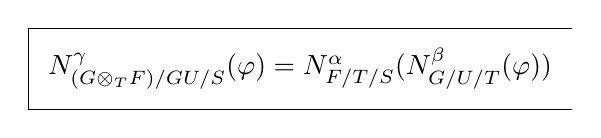
\begin{tikzpicture}
\node[inner sep=7pt] (n) {$N^\gamma_{(G\otimes_T F)/\deleted{\unsure{G}}U/S}(\varphi)=N^\alpha_{F/T/S}(N^\beta_{G/U/T}(\varphi))$};
\draw (n.north east)--(n.north west)--(n.south west)--(n.south east);
\end{tikzpicture}}
\diagram{\begin{tikzcd}[row sep=small,column sep=small]
&X_2&\\
\unsure{Y}&x\arrow[l]&\\
&X_1\arrow[d]&Y\arrow[l,"r_1"']\arrow[uul,"r_2"']\arrow[d]\\
&S&T\arrow[l]\\
&&F_1,F_2
\end{tikzcd}}
\scanpage{6}
% archive foliation: 5
% Typescript upside down in the scan; reading orientation restored here.
\begin{center}-- 35 --\end{center}
\hfill n$^{\circ}$329

PROPOSITION 10. -- \uline{La bijection canonique} $h:A/R_A\to f(A)$ \uline{est continue. En outre, les trois propriétés suivantes sont équivalentes :}

a) $h$ \uline{est un homéomorphisme} ;

b) \uline{tout ensemble ouvert dans} $A$ \uline{et saturé pour} $R_A$ \uline{est la trace sur} $A$ \uline{d'un ensemble ouvert dans} $X$ \uline{et saturé pour} $R$ ;

c) \uline{tout ensemble fermé dans} $A$ \uline{et saturé pour} $R_A$ \uline{est la trace sur} $A$ \uline{d'un ensemble fermé dans} $X$ \uline{et saturé pour} $R$.

La première partie de la proposition est immédiate (n$^{\circ}$ 5). La seconde résulte de la prop. 8 : si $B$ est un ensemble ouvert (resp. fermé) dans $A$ et saturé pour $R_A$, et si $g(B)=f(B)$ est la trace sur $f(A)$ d'un ensemble $C$ ouvert (resp. fermé) dans $X/R$, $B$ est la trace sur $A$ de l'ensemble ouvert (resp. fermé) $f^{-1}(C)$ saturé pour $R$ ; et réciproquement, si $B$ est la trace sur $A$ d'un ensemble ouvert (resp. fermé) $D$ saturé pour $R$, $f(B)$ est la trace sur $f(B)$ de $f(D)$, qui est ouvert (resp. fermé) dans $X/R$.

COROLLAIRE 1. -- \uline{Si} $A$ \uline{est un ensemble saturé pour} $R$ \uline{et ouvert} (resp. \uline{fermé}) \uline{dans} $X$, \uline{l'application canonique} $h:A/R_A\to f(A)$ \uline{est un homéomorphisme.}

En effet, si $A$ est ouvert (resp. fermé) et saturé pour $R$, et si $B\subset A$ est ouvert (resp. fermé) dans $A$ et saturé pour $R_A$, $B$ est ouvert (resp. fermé) dans $X$ et saturé pour $R$.

COROLLAIRE 2. -- \uline{S'il existe une application continue} $u:X\to A$ \uline{telle que, pour tout} $x\in X$, $u(x)$ \uline{soit congru à} $x$ mod. $R$, \uline{l'application canonique} $h:A/R_A\to f(A)$ \uline{est un homéomorphisme.}

En effet, comme toute classe d'équivalence suivant $R$ rencontre $A$, l'image canonique de $A/R_A$ dans $X/R$ est identique à $X/R$ ; d'autre part,
\scanpage{7}
% archive foliation: 6
\[\bigwedge^n M\]

a) Cas où $r=0$, $r=1$

b) Fonctorialité en $X,Y,S$
\inserted{\diagram{\begin{tikzcd}[row sep=small,column sep=small,execute at end picture={
\draw ([xshift=-8pt]\tikzcdmatrixname-1-1.north west) to[out=-90,in=90] ([xshift=-12pt]\tikzcdmatrixname-2-1.west) to[out=-90,in=150] ([xshift=-1pt]\tikzcdmatrixname-3-1.south west);
}]
\text{(i)}&X_S^{\unsure{r|n}}\arrow[r]&Y&&&\\
{}&X\arrow[r]&X'&&Y\arrow[r]&Y'\\
\text{(ii)}&F&&&F'&\\
{}&X\arrow[d]&X_S^r\arrow[r,"\varphi"]&Y&X'\arrow[d]&X_{S'}'{}^r\arrow[r,"\varphi'"]&Y'\\
{}&S&&&S'&&
\end{tikzcd}}}
\diagram{\begin{tikzcd}[row sep=small,column sep=small]
X_S^n\arrow[r,"\varphi"]\arrow[d]&Y\arrow[d]&S\arrow[l,"\unsure{\operatorname{Cor}|\operatorname{Cn}}_F^\varphi"']\\
X_S'{}^n\arrow[r,"\varphi_1"']&Y'&S\arrow[l,"\unsure{\operatorname{Cor}|\operatorname{Cn}}_{F}^{\varphi',\unsure{u}}"']
\end{tikzcd}}
\margin{\unsure{comm. polyp.}\qquad\uuline{\unsure{comm}}}
\diagram{\begin{tikzcd}[row sep=small,column sep=large]
Y&Y'\arrow[l]\\
S\arrow[u,"\unsure{\operatorname{Cor}|\operatorname{Cn}}_F^\varphi"]\arrow[r,phantom,"\text{\uuline{comm}}"]&S'\arrow[l]\arrow[u,"\unsure{\operatorname{Cor}|\operatorname{Cn}}_{F'}^{\varphi'}"']
\end{tikzcd}}

c) Additivité en $M$
\diagram{\begin{tikzcd}[row sep=large,column sep=large]
X_S^{r_1+r_2}\arrow[r,"\varphi"]&Y&S\arrow[l,"\unsure{\operatorname{Cor}|\operatorname{Cn}}_{\deleted{\unsure{F}}F_1\unsure{\oplus}F_2}^{\varphi}"']\arrow[d,equal]\\
X_S^{r_1}\times_S X_S^{r_2}\arrow[u,"\unsure{\iota}","\mathrm{can.}"']\arrow[r,"\varphi_1\times_S\varphi_2"']&Y_1\times_S Y_2\arrow[u,"u"]&\deleted{\unsure{S}}S\arrow[l,"\unsure{\operatorname{Cor}|\operatorname{Cn}}_{F_1}^{\varphi_1}\unsure{\times}\unsure{\operatorname{Cor}|\operatorname{Cn}}_{F_2}^{\varphi_2}"]
\end{tikzcd}}
\margin{\uline{comm.}\quad\deleted{\unsure{\text{polyp.}}}}

d) Transitivité.
\diagram{\begin{tikzcd}[row sep=small,column sep=small]
G&X\arrow[d]&G\otimes_Y F&\unsure{\text{Cas du}}\ \unsure{*}\\
r&Y\arrow[d]&\unsure{rs}&\\
F&Z&&\\
s&&&
\end{tikzcd}}
\diagram{\begin{tikzcd}[row sep=small,column sep=small,execute at end picture={
\draw ([xshift=-5pt,yshift=8pt]\tikzcdmatrixname-1-1.north west)--([xshift=-5pt,yshift=-5pt]\tikzcdmatrixname-4-1.south west);
\draw ([xshift=-5pt,yshift=8pt]\tikzcdmatrixname-1-1.north west)--([xshift=8pt,yshift=8pt]\tikzcdmatrixname-1-3.north east) to[out=0,in=90] ([xshift=14pt]\tikzcdmatrixname-5-3.east)--([xshift=-55pt,yshift=-8pt]\tikzcdmatrixname-5-3.south);
\draw (\tikzcdmatrixname-2-2.south) to[out=-70,in=150] (\tikzcdmatrixname-5-3.west);
\draw (\tikzcdmatrixname-1-3.south) to[out=-60,in=70] (\tikzcdmatrixname-4-3.east);
}]
X_Y^{\unsure{r}}\arrow[r,"\varphi"]&\mathcal{X}_r&\text{($Y$-\unsure{morphisme})}\\
Y_Z^s\arrow[r,"\psi"]&\mathcal{Y}_s&\text{($Z$-\unsure{morphisme})}\\
X_Z^r\arrow[r,"\unsure{f}"]&\mathcal{Z}_r&\text{($Z$-\unsure{morphisme})}\\
\mathcal{X}_Z^s\arrow[r,"u"]&\mathcal{Z}&\text{($Z$-\unsure{morphisme})}\\
&&\text{\unsure{soit comm.}}
\end{tikzcd}}
\unsure{tels que}
\diagram{\begin{tikzcd}[row sep=large,column sep=large,execute at end picture={
\draw ([xshift=-45pt,yshift=15pt]\tikzcdmatrixname-1-1.north west)--([yshift=15pt]\tikzcdmatrixname-1-1.north east);
\draw ([xshift=-45pt,yshift=15pt]\tikzcdmatrixname-1-1.north west) to[out=-85,in=70] ([xshift=-65pt,yshift=-10pt]\tikzcdmatrixname-2-1.south west) to[out=-110,in=180] ([yshift=-35pt]\tikzcdmatrixname-2-1.south) to[out=0,in=-90] ([xshift=12pt]\tikzcdmatrixname-2-2.east);
\draw ([xshift=-25pt]\tikzcdmatrixname-1-1.west) to[out=-40,in=140] (\tikzcdmatrixname-2-1.south);
}]
X_Z^{\unsure{rs}}\arrow[r,"\unsure{\gamma}"]&\mathcal{Z}\\
(X_Y^r)_Z^s\arrow[u,"\mathrm{can}"]\arrow[r,"\varphi_Z^s"']&\mathcal{X}_Z^s\arrow[u,"u"']
\end{tikzcd}}
\margin{\unsure{commutatif}}
\scanpage{8}
% archive foliation: 7
% Typescript upside down in the scan; reading orientation restored here.
\begin{center}-- 37 --\end{center}
\hfill n$^{\circ}$329

assertion. On observera que $A/R_A$ s'obtient en identifiant dans $A$ les points 0 et 1. $*$

\begin{center}§ 4. Produit d'espaces topologiques.\end{center}

1. \uline{Espaces produits}

DEFINITION 1. -- \uline{Etant donnée une famille} $(X_i)_{i\in I}$ \uline{d'espaces topologiques, on appelle espace produit de cette famille l'ensemble produit} $X=\prod_{i\in I}X_i$ \uline{muni de la topologie produit des topologies des} $X_i$ (§ 2, n$^{\circ}$3, \uline{Exemple} III). \uline{On dit que les} $X_i$ $(i\in I)$ \uline{sont les espaces facteurs de} $X$.

En vertu du § 2, n$^{\circ}$ 3, prop. 4, la topologie produit sur $X$ a pour \uline{base} l'ensemble \uline{$B$} des intersections \uline{finies} d'ensembles de la forme $\operatorname{pr}_i^{-1}(U_i)$ où $U_i$ est ouvert dans $X_i$ ; ces ensembles ne sont autres que les produits $\prod_{i\in I}A_i$, où $A_i$ est \uline{ouvert} dans $X_i$ pour tout $i\in I$ et où $A_i=X_i$ \uline{sauf pour un nombre fini d'indices} ; nous donnerons à ces ensembles le nom \uline{d'ensembles élémentaires.} Si \uline{$B_i$} est une base de la topologie de $X_i$ (pour tout $i\in I$), il est clair que les ensembles élémentaires $\prod_{i\in I}A_i$ tels que $A_i\in\text{\uline{$B_i$}}$ pour tout $i$ tel que $A_i\ne X_i$ forment encore une \uline{base} de la topologie produit. Ceux de ces ensembles qui contiennent un point $x\in X$ forment par suite un \uline{système fondamental de voisinages} de $x$ (§ 1, n$^{\circ}$3, prop. 3).

Lorsque $I$ est un ensemble \uline{fini}, la construction de la topologie produit à partir des topologies des $X_i$ se simplifie : les ensembles élémentaires sont simplement les produits $\prod_{i\in I}A_i$, où $A_i$ est une partie ouverte quelconque de $X_i$ pour \uline{tout} $i\in I$ (cf. exerc.\quad).

\uline{Exemples.} -- $*$ Le produit $\unsure{\text{\uline{$R$}}|\text{\uline{$F$}}}^n$ de $n$ espaces identiques à la droite
\scanpage{9}
% archive foliation: 8
\diagram{\begin{tikzcd}[column sep=large]
G_Z^{rs}\arrow[r,"\varphi","\text{symm}"']&G'
\end{tikzcd}}
d'où diag. comm.
\diagram{\begin{tikzcd}[row sep=small,column sep=large]
(G_Y)_Y^{\unsure{rs}}\arrow[r,"\varphi_Y"]\arrow[d,no head]&G'_Y\arrow[d,"c"]\\
G_Z^{\unsure{rs}}\arrow[r,"\varphi"']&G'
\end{tikzcd}}

On suppose qu'on a aussi
\diagram{\begin{tikzcd}[column sep=large]
(G_Y)^r\arrow[r,"\psi","\text{symm}"']&G''
\end{tikzcd}}
\margin{\deleted{\unsure{d'où}}}
\deleted{$(\unsure{G_Y})^{\unsure{r}}-$}
\diagram{\begin{tikzcd}[column sep=large]
G_Z''{}^s\arrow[r,"\chi","\text{symm}"']&G'\deleted{\unsure{_Y}}
\end{tikzcd}}
\margin{\uline{$Z$-\unsure{morphisme}} \unsure{rendant commutatif}}
\diagram{\begin{tikzcd}[row sep=large,column sep=large]
(G_Y)^{rs}\arrow[r,"\psi_Y^s"]\arrow[dr,"\unsure{\mathrm{can.}\varphi_Y}"']\arrow[d,"\deleted{\unsure{\varphi}}"']&G_Z''{}^s\arrow[d,"\chi"]\\
\deleted{\unsure{G'}}&G'\deleted{\unsure{_Y}}
\end{tikzcd}}

Considérons : $\alpha:X\to G$ un $Z$-morphisme, d'où
\[
N^\varphi_{G/X/Z}(\alpha):Z\longrightarrow G'
\]
\margin{\unsure{lié par} $\alpha=c\alpha'$\quad $\alpha':X-G_Y$, d'où}
Mais aussi un $Y$-morphisme
\[
N^\psi_{G/X/Y}(\alpha'):Y\longrightarrow G''
\]
et \unsure{par suite}, en appliquant $\chi$, un morphisme
\[
N^\chi_{F/Y/Z}\bigl(N^\psi_{G/X/Y}(\alpha')\bigr):Z\longrightarrow G'
\]
Je dis qu'on a
\[
\boxed{N^\varphi_{G/X/Z}(c\alpha')=N^\chi_{F/\unsure{X|Y}/Z}\bigl(N^\psi_{G/X/Y}(\alpha')\bigr)}
\]
\scanpage{10}
% archive foliation: 9
% Typescript upside down in the scan; reading orientation restored here.
\begin{center}-- 36 --\end{center}
\hfill n$^{\circ}$329

si $U$ est ouvert dans $A$ et saturé pour $R_A$, il résulte de l'hypothèse que $u^{-1}(U)$ est identique à l'ensemble obtenu en saturant $U$ pour $R$ ; comme $u$ est continue, $u^{-1}(U)$ est ouvert dans $X$ (§ 2, n$^{\circ}$1, th. 1) d'où le corollaire, en vertu de la prop. 10.

Exemples. -- 1) Soit $X$ un espace somme d'une famille $(X_i)_{i\in I}$ d'espaces topologiques, identifiés canoniquement à des sous-espaces de $X$, et considérons l'espace quotient $X/R$ obtenu par \uline{recollement} des $X_i$ le long de sous-ensembles $A_{i\unsure{x|\varkappa}}$ au moyen de bijection $h_{i\unsure{x|\varkappa}}$ (n$^{\circ}$4, \uline{Exemple} 1). Soit $f$ l'application canonique $X\to X/R$ ; sa restriction à chaque $X_i$ est par hypothèse une bijection continue de $X_i$ sur le sous-espace $f(X_i)$ de $X/R$ ; cherchons si cette application peut être un \uline{homéomorphisme} quel que soit $i\in I$. Puisque $f(A_{i\unsure{x|\varkappa}})=f(A_{\unsure{x|\varkappa}i})$, une condition \uline{nécessaire} est que $h_{i\unsure{x|\varkappa}}$ soit un homéomorphisme quels que soient $i$ et $\unsure{x|\varkappa}$. Mais cette condition \uline{n'est pas suffisante} en général (exerc.\quad). Elle l'est toutefois dans le cas important où les $A_{i\unsure{x|\varkappa}}$ sont tous \uline{ouverts} ou tous \uline{fermés.} En effet, supposons par exemple que les $A_{i\unsure{x|\varkappa}}$ soient tous fermés ; si $F$ est un ensemble fermé quelconque dans $X_i$, $h_{i\unsure{x|\varkappa}}(F\cap A_{i\unsure{x|\varkappa}})$ est fermé dans $X_{\unsure{x|\varkappa}}$ ; or, pour saturer $F$ pour $R$, il faut prendre la réunion de tous les ensembles $h_{i\unsure{x|\varkappa}}(F\cap A_{i\unsure{x|\varkappa}})$ (pour $\unsure{x|\varkappa}\in I$) ; on obtient ainsi un ensemble fermé dans $X$ en vertu du § 1, n$^{\circ}$5, prop. 4, et notre assertion résulte donc de la prop. 10. Le raisonnement est analogue si les $A_{i\unsure{x|\varkappa}}$ sont ouverts.

$*$ 2) Désignons par $R$ la relation d'équivalence $x\equiv y$ (mod.1) dans la droite numérique \uline{$R$} (n$^{\circ}$4, Exemple 2), par $A$ l'intervalle fermé $[0,1]$ ; $A$ contient un point au moins de toute classe d'équivalence suivant $R$. L'application canonique de $A/R_A$ sur le tore \uline{$T$} est un homéomorphisme ; en effet, soit $F$ un ensemble fermé dans $A$ (donc dans \uline{$R$}) ; pour saturer $F$ pour la relation $R$, il faut prendre la réunion des ensembles fermés $F+n$ (pour $n\in\text{\uline{$Z$}}$), qui forment évidemment une famille localement finie ; leur réunion est donc fermée (§ 1, n$^{\circ}$5, prop. 4), d'où notre
\scanpage{11}
% archive foliation: 10
\uline{Théorie axiomatique des morphismes \unsure{normés|normants}}

Soit $C$ une catégorie, \inserted{\unsure{où les sommes finies existent}}, et soit $\mathcal{N}$ un ensemble de morphismes dans $C$, \deleted{appelés \unsure{morphismes normés}}, ayant les propriétés suivantes

(i) Si $X\in C$, alors $\operatorname{id}_X\in\mathcal{N}$

(ii) Si $u,v\in\mathcal{N}$ sont composables, alors $vu\in\mathcal{N}$

(iii) Si $u:X\longrightarrow Y$ est dans $\mathcal{N}$, et si $Y'\to Y$ est quelconque, alors $X'=X\times_Y Y'$ existe et $u^{Y'}:\deleted{\unsure{X\times_Y}}X'\to Y'$ est $\in\mathcal{N}$

(iv) Si $u_i:X_i\to Y$ $(i=1,2)$ sont $\in\mathcal{N}$, alors $(u_1,u_2):X_1\amalg X_2-Y$ est dans $\mathcal{N}$ ; de plus, l'\unsure{existence} de \unsure{la} \illegible{1} \inserted{$\unsure{\prod}$ et $\unsure{\coprod}$} \unsure{compatible à la formation de} \unsure{sommes}

(v) Si $u:X\to Y$ est $\in\mathcal{N}$, alors \inserted{$\forall n$ \unsure{tout} ss-groupe $G$ de $\unsure{\mathfrak{S}_n|\mathcal{S}_n}$,} le quotient $(\overbrace{X\times_Y\cdots\times_Y X}^{n\text{ fois}})/G$ existe, \inserted{\unsure{et est comp. aux changements de base}}\margin{\unsure{!|?}}

\deleted{\unsure{Il est clair que}}
Soit $\deg$ une fonction sur $\mathcal{N}$, \inserted{notation aussi : $\deg(X/Y)$,} ayant les propriétés suivantes

(i bis) $\deg(\operatorname{id}_X)=1$

(ii bis) $\deg(vu)=\deg v\,\deg u$

(iii bis) $\deg(u)=\deg(u^{Y'})$

(iv bis) $\deg(u,v)=\deg u+\deg v$

(v bis) Le quotient considéré dans (v) a \uuline{\unsure{un}} degré \deleted{\unsure{fini}} \unsure{se calcule} ainsi : Soit \deleted{$\unsure{r=\deg(X/Y)}$}\inserted{$r=\deg(X/Y)$}, $\unsure{A}$ \inserted{$E=[1,r]$},
\deleted{$E=\Delta^r,\quad F=(\mathop{\otimes}\nolimits^r E)/G$ \unsure{deux} \illegible{3}}
Soit $F=E^n/G$, alors \deleted{$\unsure{\deg(X/Y)^n/G}$} le degré de $(\underbrace{X\times_Y-\times_Y X}_{n})/G$ est égal à $\operatorname{card}(E^n/G)$.

Enfin, pour \deleted{\unsure{tout}} morphisme $u\in\mathcal{N}:X-Y$ \inserted{de degré $r$}, \unsure{sur}\ $\mathcal{N}$- soit donné un morphisme
\[
\unsure{\operatorname{Cor}|\operatorname{Cn}}_u=\unsure{\operatorname{Cor}|\operatorname{Cn}}_{X/Y}:Y-\Sigma^r X
\]
(\inserted{appelé} \deleted{\unsure{noté}} \uline{norme} de $u$, ou de $X/Y$), avec les propriétés suivantes

(i ter) $\unsure{\operatorname{Cor}|\operatorname{Cn}}_{X/X}=\operatorname{id}_X$

(ii ter) La commutativité dans le diagramme suivant :
\scanpage{12}
% archive foliation: 11
(où $X\xrightarrow[r]{u}Y\xrightarrow[s]{v}Z$ sont des morphismes $\in\mathcal N$, de degré $r,s$) :
\diagram{\begin{tikzcd}Y\arrow[r]&\Sigma^r(X/Y)\end{tikzcd}}
\diagram{\begin{tikzcd}[column sep=large,row sep=large]
Z\arrow[r,"{\unsure{\operatorname{Cor}|\operatorname{Cn}}_{Y/Z}}"']\arrow[rrd,"{\deleted{\unsure{\longrightarrow}}}" description]\arrow[rrdd,"{\unsure{\operatorname{Cor}|\operatorname{Cn}}_{X/Z}}"]\arrow[rrddd,"{\deleted{\unsure{\longrightarrow}}}" description]&\Sigma^s(Y/Z)\arrow[r,"{\Sigma^s(\unsure{\operatorname{Cor}|\operatorname{Cn}}_{X/Y}/Z)}"]&\Sigma^s(\Sigma^r(X/\unsure{Y})/Z)\arrow[d,"{\mathrm{can}}"]\\
&&\Sigma^s(\Sigma^r(\deleted{\unsure{X}}X/Z)/Z)\arrow[d,"{\mathrm{can}}"]\\
&&\Sigma^{sr}(X/Z)\\
&&{}
\end{tikzcd}}

(iii ter) Soit $u:X\longrightarrow Y$ dans $\mathcal N$, et $Y'\longrightarrow Y$ quelconque, alors $\unsure{\operatorname{Cor}|\operatorname{Cn}}_{X'/Y'}\deleted{Y'\longrightarrow}$ est ``image réciproque'' de $\unsure{\operatorname{Cor}|\operatorname{Cn}}_{X/Y}$ par $Y'\longrightarrow Y$, i.e. le diagramme
\diagram{\begin{tikzcd}
\Sigma^r(X/Y)&Y\arrow[l,"{\unsure{\operatorname{Cor}|\operatorname{Cn}}_{X/Y}}"']\\
\Sigma^r(X'/Y')\arrow[u,"{\mathrm{can}}"]&Y'\arrow[l,"{\unsure{\operatorname{Cor}|\operatorname{Cn}}_{X'/Y'}}"']\arrow[u]
\end{tikzcd}}
est commutatif

(iv ter) Soient $u_i:\deleted{\unsure{X}}X_i\longrightarrow Y\quad(i=1,2)$ dans $\mathcal N$. Soit $X=X_1\amalg X_2$, $u=(u_1,u_2)$ ; donc pour $\forall$ entier $r$, on a
\[
\Sigma^r(X/Y)=\deleted{\unsure{\Pi}}\coprod_{\substack{i+j=r\\i,j\geq0}}\Sigma^i(X_1/Y)\times\Sigma^j(X_2/Y)
\]
en particulier, si $r_i=\deg u_i$ et $r=r_1+r_2=\deg u$, on a un morphisme \inserted{\unsure{d'injection|d'immersion}} canonique $\Sigma^{r_1}(X_1/Y)\times\Sigma^{r_2}(X_2/Y)\longrightarrow\Sigma^r(X/Y)$. Ceci dit, on a commutativité du
\diagram{\begin{tikzcd}[column sep=large]
Y\arrow[r,"{(\unsure{\operatorname{Cor}|\operatorname{Cn}}_{X_1/Y},\unsure{\operatorname{Cor}|\operatorname{Cn}}_{X_2/Y})}"]\arrow[rd,"{\unsure{\operatorname{Cor}|\operatorname{Cn}}_{X/Y}}"']&\Sigma^{r_1}(X_1/Y)\times\Sigma^{r_2}(X_2/Y)\arrow[d]\\
&\Sigma^r(X/Y)
\end{tikzcd}}

\uline{Exemple I} Soit $G$ un groupe, soit $C$ la catégorie des ensembles où $G$ opère. Un morphisme $u:X\longrightarrow Y$ de $C$ sera \deleted{dans $\mathcal N$ s'il existe} \inserted{dit de degré $r$} \deleted{\unsure{$r$ tel que pour $\forall$}} si pour $\forall\ y\in Y$, \deleted{\unsure{il y a}} \deleted{\illegible{2}} $\operatorname{card}(u^{-1}(y))=r$. Un morphisme est dans $\mathcal N$ s'il existe $r$ tel qu'il soit de degré $r$. Les conditions (i) ; (v) et (i bis) ; (v bis) sont trivialement vérifiées. [N.B. les produits fibrés et sommes à ens d'indices quelconque existent dans $C$, \deleted{\unsure{et}} de $=$ le quotient d'un objet de $C$ par un groupe d'automorphismes $\unsure{G|H}$]. Soit $u:X-Y$ de degré $r$. Notons que $\Sigma^r(X/Y)$ est l'ensemble \inserted{comme ens. sous-jacent} \deleted{\unsure{des $r$-uplets}} réunion des $\Sigma^r(u^{-1}(y))\quad(y\in Y)$ ; comme $u^{-1}(y)$ a exactement $r$ \unsure{éléments}, \unsure{Alors}, \deleted{\unsure{il}} il y a dans $\Sigma^r(u^{-1}(y))$ un élément privilégié, \unsure{(image} du $r$-uplet \inserted{mod $\mathfrak{S}_r$} de ces $r$ éléments rangés dans un ordre quelconque). D'où une application-section $Y\longrightarrow\Sigma^r(X/Y)$, qui évidemment permute aux automorphismes de la situation, donc : \unsure{fonctorielle}, \unsure{i.e.} \deleted{\unsure{un}} c'est un \deleted{\unsure{hom}} hom de $C$. Si on
\scanpage{13}
% archive foliation: 12
la désigne par $\unsure{\operatorname{Cor}|\operatorname{Cn}}_{X/Y}$, on vérifie aussitôt les conditions (i ter) : (iv ter).

\margin{Expliquer la relation de cet exemple avec le cas général, peut-on en \unsure{déduire} \uline{\unsure{galoisiennes}} \uline{\unsure{spéciales}} \uline{\unsure{par un autre}}}

\uline{Exemple II} Soit $C$ la catégorie des schémas \inserted{(dans un univers donné)}. Un morphisme fini et plat \inserted{$u:X\longrightarrow Y$} est dit de \uline{degré $r$} s'il correspond à un \deleted{\unsure{bon}} faisceau \deleted{cohérent de} \inserted{\unsure{qu. coh.}} \unsure{d'algèbres} sur $Y$, loc. libre de \deleted{degré} rang $r$ en $\forall$ point. Soit $\mathcal N$ l'ensemble des morphismes qui sont finis et plats et ont un \deleted{\unsure{un}} degré $r$. Les conditions (i) : (v) et (i bis) : (v bis) sont vérifiées, comme on voit \deleted{aussitôt} très facilement. \deleted{De} Plus, on peut définir de façon naturelle \uline{des} \deleted{applications} morphismes $\unsure{\operatorname{Cor}|\operatorname{Cn}}_{X/Y}$, satisfaisant les conditions (i) : (iv).

\uline{Exemple III \deleted{\unsure{Variantes}}} \inserted{(Variantes)} En géométrie analytique, on a une variante directe. En topologie, prenant les revêtements \unsure{non ramifiés} \deleted{de} \inserted{ayant un} degré, on trouve une variante analogue ; elle est très proche de l'exemple I, \deleted{\illegible{2}} \inserted{de façon} précise, soit $X$ un espace topologique \uline{fixé}, \deleted{prenons les} Alors
\scanpage{14}
% archive foliation: 13
Soit $X\in C$, avec un groupe $\unsure{\Gamma|G}$ d'automorphismes \inserted{à droite}. On suppose que pour $\forall$ sous-groupe $H$ de $G$, \deleted{et $\forall$ \illegible{1}} $X/H$ existe, et que pour $H'\subset H$ \inserted{invariant} d'indice fini $r$ dans $H$, \deleted{$X/H'\longrightarrow X/H$ soit dans $(\mathcal N)$ et de degré $r$. (on a encore des exemples, et des \illegible{2}, pour les)} \unsure{l'objet|le couple} $X/H'$ avec groupe à opérateurs fini $H/H'$ soit \uline{non ramifié}, et $X/H'\longrightarrow X/H=(X/H')/(H/H')$ est $\in(\mathcal N)$. Soit $C'$ la catégorie des ensembles $E$ où $\Gamma$ opère, et pour $E/\Gamma$ soit fini. Alors \deleted{\unsure{pour}} pour $\forall\ E\in C'$, $X\times_{(\Gamma)}E$ \uline{existe}, soit $\Phi(E)=X\times_{(\Gamma)}E$,

\margin{\uuline{\unsure{à développer}}}
\figure{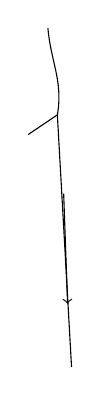
\begin{tikzpicture}\draw (0,0) to[out=-85,in=80] (0.12,-1.1)--(0.3,-4.3);\draw (0.12,-1.1)--(-0.25,-1.35);\draw[->] (0.2,-2.1)--(0.25,-3.5);\end{tikzpicture}}
$\Phi$ est donc un foncteur $\unsure{C'|E'}\longrightarrow C$, commutant aux sommes finies, et on sait de plus que $\Phi$ transforme morphisme de degré $r$ en morphisme de degré $r$ (\unsure{id : fait aussi sur} $\mathcal N$). De plus, il transforme \deleted{morphismes} \inserted{conserve} les \unsure{compos}\ldots
\scanpage{15}
% archive foliation: 14
\begin{center}- 99 -\end{center}\hfill n\textsuperscript{o} 268

points génériques indépendants de $A$, on a
\[
s_m(u_1,\ldots,u_m)=u_1+\cdots+u_m\,.
\]
Onnotera $p_i:A_{(m)}\longrightarrow A_i$ la projection sur le i-ème facteur. Si $X$ est un diviseur sur $A$, alors $p_i^{-1}(X)$ est égal au diviseur $A\times\cdots\times X\times\cdots\times A$, avec $X$ au lieu de $A$ au i-ème facteur.

\uline{Théorème} 6 - Soit $X$ un diviseur sur $A$. Alors $X\equiv0$ si et seulement si $s_m^{-1}(X)\sim\sum_{i=1}^m p_i^{-1}(X)$.

\uline{Démonstration} - Pour simplifier les notations, prenons $m=2$. Pour $u$ générique sur $A$, on a
\[
s_2^{-1}(X).(A\times u)=X_{-u}\times u
\]
et par conséquent
\[
[s_2^{-1}(X)-X\times A].(A\times u)=(X_{\unsure{-1|-u}}-X)\times u.
\]
Si $X\equiv0$, on a d'après le principe de la balançoire (Appendix, th. 6)
\[
s_2^{-1}(X)-X\times A\sim A\times Y
\]
avec un diviseur $Y$ convenable. Par symétrie, on doit avoir $Y\sim X$. La réciproque est évidente.

\uline{Corollaire} - Soient $\alpha:A\longrightarrow B$ et $\beta:A\longrightarrow B$ deux homomorphismes d'une variété abélienne $A$ dans une variété abélienne $B$, et soit $X$ un diviseur sur $B$, $X\equiv0$, et soit $\xi=\operatorname{Cl}(X)$. Soient $\alpha^{-1}$, $\beta^{-1}$ les applications induites de $D(B)/D_\ell(B)$ dans $D(A)/D_\ell(A)$. Alors on a
\[
(\alpha+\beta)^{-1}(\xi)=\alpha^{-1}(\xi)+\beta^{-1}(\xi).
\]
En particulier, si $A=B$ et $n$ est un entier, on a
\[
(n\delta)^{-1}(\xi)=n\xi.
\]
\uline{Démonstration} . - Soit $\lambda=(\alpha,\beta)$ l'application composée de $A$ dans $B\times B$, i.e. L'application $\lambda(u)=(\alpha(u),\beta(u))$, et soit $s_2$ la somme sur $B$. On a $\alpha+\beta=s_2\lambda$.
\diagram{\begin{tikzcd}A\arrow[r,"\lambda"]&B\times B\arrow[r,"s_2"]&B\end{tikzcd}}
\scanpage{16}
% archive foliation: 15
Soit $G$ un groupe, $C_G$ la catégorie des ensembles $E$ où $G$ opère \inserted{à \deleted{droite} gauche}, et tels que $E/G$ soit fini. On sait que la catégorie des hyperfaisceaux d'ensembles sur $C_G$ (\deleted{pour} les épimorphismes dans $C_G$ comme morphismes de descente) est équivalente à la catégorie des ensembles \deleted{(quelconques)} où $G$ opère à \deleted{droite} \inserted{gauche} ; si $A$ est un tel, $\Phi_A$ l'hyperfaisceau associé, on a
\margin{à développer}\figure{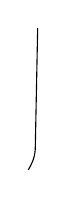
\begin{tikzpicture}\draw (0,0)--(-0.03,-1.5) to[out=-90,in=60] (-0.12,-1.8);\end{tikzpicture}}
\[
\Phi_A(\deleted{\unsure{E}}X)=\deleted{A\times_{(G)}\unsure{X}\times_{(G)}A}\operatorname{Hom}_G(X,E)
\]
\deleted{Ainsi, \unsure{étant donné}, la \unsure{donnée}\unsure{?}}

Et si $\Phi$ est un hyperfaisceau, alors l'ensemble à opérateurs associé est
\[
A=\Phi(G_g)
\]
où $G_g$ désigne $G$ considéré comme ens. à groupe d'opérateurs à gauche $G$ par l'op. rég. gauche.

\deleted{Soit $F$ un sous-groupe de $G$, et soit $C_{G;F}$ la sous-catégorie de $C_G$ formée des $X\in C_G$ tels que $F$ y opère \unsure{trivialt} ; c'est une sous-catégorie stable pour les opérations habituelles [sommes, \unsure{lim}, produits fibrés, quotients et \unsure{foncteurs} $\operatorname{Hom}$].}
\scanpage{17}
% archive foliation: 16
\begin{center}- 94 -\end{center}\hfill n\textsuperscript{o} 268

construction, et c'est donc un homomorphisme (Chap.I, \S 1). On notera que si $A$ est complète, $B$ l'est aussi.

De plus, le diviseur $\overline{D(u)}$ étant rationnel sur $k(f(u))$, il existe un diviseur positif $E$ sur $B\times V$ tel que $\overline{D(u)}=E(f(u))$ (par F-VII$_6$ th.12). Les conditions (i) et (ii) sont alors évidemment satisfaites La conditions (iii) est précisément ce que nous avons démontré dans le lemme et la condition (iv) est celle que nous venons d'obtenir.

Le corollaire 1 - est alors facile à démontrer. Je dis que le noyau de $f$ est égal au noyau de l'homomorphisme
\[
w\longrightarrow\operatorname{Cl}[D(w+v)-D(v).]
\]
En effet, si $D(a+v)-D(v)\sim0$ avec $a\in A$, et $v$ générique sur $k(a)$, alors $f(a+v)=f(v)$, et par conséquent $f(a)=0$. Réciproquement, si $f(a)=0$, alors pour $v$ générique sur $k(a)$, $f(a+v)=f(v)$ et $E(f(a+v))=E(f(v))$, autrement dit $\overline{D(a+v)}=\overline{D(v)}$. Cela donne bien $D(a+v)-D(v)\sim0$, et termine notre discussion du quotient dans le théorème du carré.

4 - \uline{Applications du théorème du carré aux variétés abéliennes.}

Dans ce numéro, nous allons employer le fait que la variété de groupe est complète pour obtenir des résultats plus précis sur l'application $\varphi_X:a\longrightarrow\operatorname{Cl}(X_a-X)$ définie à la fin du numéro précédent.

Nous dirons qu'un diviseur $X$ sur une variété abélienne $A$ est \uline{non dégénéré} si le noyau de $\varphi_X$ est fini. Nous démontrerons au cours du chapitre les résultats suivants : Il existe des diviseurs non dégénérés, et pour de tels diviseurs, l'application $\varphi_X$ est surjective. Il existe un entier $d$ dépendant de $A$ seulement, tel que pour n'importe quel diviseur $Y$ on ait $\varphi_Y=0$ si et seulement si $dY$ est algébriquement équivalent à $0$. Pour définir ensuite la
\scanpage{18}
% archive foliation: 17
\[\text{\textcircled{A}}\qquad\boxed{H^{\unsure{*}}(G,A)\Longleftarrow H^p(T/e,\underline{\mathcal H}^{q}(A))}\qquad(T\ne\varnothing)\]
\margin{\unsure{s'apparente} à la suite spectrale de Leray d'un \uline{recouvrement} d'un espace}
où $\underline{\mathcal H}^{q}(A)$ est le \unsure{pré}\uuline{pré}faisceau sur $C_G$ \deleted{défini par $\underline{\mathcal H}^{q}(A)(G/F)=H^q(F,A)$} dont la valeur sur $S\in C_G$ est donnée par
\[
\underline{\mathcal H}^{q}(A)(S)=R_A^q\deleted{\unsure{R}}(\operatorname{Hom}_{G}(S,A))
\]
[ et est donc défini aussi par les conditions de \deleted{\unsure{permuter aux}} transformer sommes \inserted{finies} en produits, et d'être donné, pour $S=F\backslash G$, par $\mathcal H^q(A)(F\backslash G)=H^q(F,A)$ ]

\unsure{Preuve.} \unsure{utiliser} essentiellement les faits suivants

(i) $T\longrightarrow e$ est un morphisme de descente, en particulier \deleted{\unsure{$H^0$}} pour un hyperfaisceau $\Phi$, on a
\[
\Phi(e)=H^0(T/e,\Phi)
\]
(ii) Si $\Phi$ est \inserted{un hyperfaisceau} injectif, alors $H^p(T/e,\Phi)=0$ pour $p>0$ (il suffit de faire $\Phi=\Phi_A$ avec $A=\operatorname{Hom}_{Z}(Z(G),M)=M^G$, alors $\Phi(S)=$ fonc des applications de $S$ dans $M$ ; donc
\[
H^p(T/e,\Phi)=H^p(\text{complexe de \unsure{simplexe} \unsure{simple} défini par }T\ ;\ M)=\unsure{0}
\]
qui est nul si $p>0$.
\scanpage{19}
% archive foliation: 18
\begin{center}- 90 -\end{center}\hfill n\textsuperscript{o} 268

nous pouvons supposer que $P\notin\operatorname{supp}(D)$. Soit $f_0,\ldots,f_n$ une base de $L(D)$ telle que toutes les fonctions $f_i$ soient définies sur $K$. Toute fonction $f\in L(D)$ peut être écrite
\[
f=f_\lambda=\sum_{i=0}^n\lambda_i f_i\qquad\lambda_i\in\Omega\,.
\]
Puisque aucun des $f_i$ n'a de pôle passant par $P$, chaque $f_i$ est dans $\unsure{\mathfrak{o}|v}$ (IAG) et a une expension en série de puissance
\[
f_i=\sum_{\mu=0}^{\infty}c_{i\mu}M_\mu(t)\qquad c_{i\mu}\in K
\]
et par conséquent
\[
f_\lambda=\sum_{\mu=0}^{\infty}\left(\sum_{i=1}^n\lambda_i c_{i\mu}\right)M_\mu(t).
\]
La matrice infinie $\|c_{i\mu}\|$ est de rang $n+1$ parce que les $f_i$ sont linéairement indépendantes sur $K$. Soit $s$ le plus petit entier tel que $\|c_{i\mu}\|\quad i=0,\ldots,n\quad\text{et}\quad\mu=0,\ldots,s$ soit de rang $n+1$. Alors les équations
\[
\sum_{i=0}^n\lambda_i c_{i\mu}=0\qquad\mu=0,\ldots,s
\]
déterminent les $\lambda_i$ de façon unique dans $K$ (à un facteur d'homogénéité près). La fonction correspondante $f_\lambda$ a un diviseur
\[
(f_\lambda)=X-D\qquad X>0.
\]
Puisque $f_\lambda$ est rationnelle sur $K$, il s'ensuit que $X$ est rationnel sur $K$. Il est clair d'après la construction que le diviseur $X$ est le diviseur dont on a démontré l'unicité dans (i). Ceci démontre notre \deleted{théorème.} \inserted{\unsure{prop}}

\uline{Théorème} - Soit $D$ un diviseur positif sur un produit $A\times V$ d'une variété de groupe commutatif et d'une variété $V$ \uline{complète sans singularités de codimension 1}. Soit $k$ un corps de définition pour $A$ et $V$, sur lequel $D$ soit rationnel, et tel que $V$ possède \uline{un point simple $P$ rationnel sur $k$}. Alors il existe une variété de groupe commutatif $B$ et un
\margin{\unsure{utile au cas non singulier?}}
\margin{\unsure{Nouveau!|Revoir!}}
\scanpage{20}
% archive foliation: 19
Plus généralement \deleted{on} posons
\[
\mathcal H^q(\Phi)(S)=H^q(-/S,\Phi)=\left\{\begin{gathered}\text{valeur en }\Phi\text{ du}\\\text{foncteur dérivé qième}\\\text{de }\Phi\longrightarrow\Phi(S)\end{gathered}\right.
\]
\margin{\unsure{identités} à développer $\longrightarrow$}
\inserted{définition \unsure{valeur en} $\Phi|S$ \unsure{du foncteur dérivé} de $\Gamma^S$ sur la catégorie des \deleted{\unsure{hyperfaisceaux}} \unsure{hyperfaisceaux} au dessus de $S$ ; \unsure{il en résulte immédiatement}}

\figure{\begin{tikzpicture}\draw (0,0) to[out=-100,in=100] (0.12,-0.55) to[out=-80,in=120] (0.5,-2.7);\end{tikzpicture}}
On sait que

(i) $\mathcal H^q(\Phi)$ est un hyper-préfaisceau qui \deleted{\unsure{transforme}} transforme sommes \inserted{finies} en produits

(ii) $\mathcal H^q(\Phi_A)(G/F)=H^q(F,A)$

Sous ces conditions, on a la suite spectrale suivante, si $T\longrightarrow S$ est \uline{surjectif} (dans $C_G$)
\[
\text{\textcircled{B}}\qquad\boxed{H^*(-/S,\Phi)\Longleftarrow H^p(T/S,\mathcal H^q(\Phi))}
\]
\margin{\fbox{\parbox{3cm}{suite spectrale de Leray - Čech}}}

Si $F'\subset F\subset G$, on peut prendre $T=G/F'\qquad S=G/F$ et on obtient, si $A$ est un $G$-module
\[
H^*(F,\deleted{\unsure{\Phi}}A)\Longleftarrow H^p(F^{\unsure{\natural|n}}_{\mathrm{mod}\,F'};\mathcal H^q(\deleted{\unsure{\Phi}}A))
\]
La suite spectrale est la $=$ que si on oublie sur $A$ la structure de $G$-module, et on retient que celle de $F$-module. La suite spectrale \textcircled{B} n'est donc pas essentiellement plus générale que \textcircled{A}.

\margin{$\Vert$ Tout ceci est à généraliser aux hyperfaisceaux quelconques \quad -- -- -- -- --}
\scanpage{21}
% archive foliation: 20
\begin{center}- 89 -\end{center}\hfill n\textsuperscript{o} 268

et si $f$, $f'$ sont deux fonctions telles que $(f)=X-X_0$;

et $(f')=X'-X_0$, il faut montrer que pour toute constante $c$, le diviseur $X_c$ tel que $(f+cf')=X_c-X_0$ est dans $\mathcal L_N$. Soit $g$ une fonction et $Y$ un diviseur tels que $X_0=(g)+Y$, et que $P\notin\operatorname{supp}(Y)$. Alors on a $(fg)=X-Y$ et $(f'g)=X'-Y$.

Ceci montre que $fg$ et $f'g$ sont dans $I_N$, donc que $(f+cf')g$ est dans $I_N$ On a évidemment
\[
(f+cf')g=X_c-Y.
\]
et par définition, on voit que $X_c$ satisfait aux conditions $I_N$. Ceci démontre que $\mathcal L_N$ est un système linéaire. Pour $N$ suffisamment grand, on voit tout de suite que $\mathcal L_N$ est vide. Quant au fait que la dimension baisse au plus d'une unité quand $N$ augmente.d'une unité, c'est clair.

\uline{Proposition} - Soit $\mathcal L$ un système linéaire \uline{complet}, et $\{I_N\}$ un système de conditions linéaires en un point simple $P$ de $V$. Alors :

(i) Il existe un entier $N(\geq-1)$ uniquement déterminé par la propriété suivante : Au moins un diviseur $X$ de $\mathcal L$ satisfait les condition $I_N$ et aucun diviseur de $\mathcal L$ ne satisfait aux conditions $I_{N+1}$. Pour cet entier $N$, il existe un diviseur $X$ et un seul de $\mathcal L$ satisfaisant $I_N$.

(ii) Si $V$ est définie sur $k$, $P$ rationnel sur un corps $K\supset k$, et s'il existe un diviseur $D$ sur $V$, rationnel sur $K$, linéairement équivalent aux diviseurs de $\mathcal L$, alors le diviseur unique $X$ du (i) est rationnel sur $K$.

\uline{Démonstration} - Le (i) est une conséquence immédiate de la proposition qui précède. Passons au (ii). En employant le fait que tout diviseur est localement linéairement équivalent à $0$ en un point simple,
\scanpage{22}
% archive foliation: 21
\[H^*(-/S,G_m)\Longleftarrow\]
\[\deleted{\cdot\quad H^2(-/S,G_m)}\]
\diagram{\begin{tikzcd}[column sep=small,row sep=large,execute at end picture={\draw ([xshift=-3mm,yshift=5mm]\tikzcdmatrixname-1-1.north west) rectangle ([xshift=5mm,yshift=-5mm]\tikzcdmatrixname-3-4.south east);}]
\unsure{\bullet|0}\arrow[r]&H^2(T/S,G_m)\arrow[r]&H^2(-/S,G_m)\arrow[r]&H^0(T/S;\mathcal H^2(G_m))\arrow[d,"d_3"]\\
&&&H^3(T/S,G_m)\arrow[d]\\
&&&H^3(-/S,G_m)'\arrow[d]\\
&&&H^1(T/S,\mathcal H^2(G_m))\arrow[d,"d_3"]\\
&&&H^4(T/S,\deleted{\unsure{\mathcal H}}G_m)\arrow[d]\\
&&&\deleted{\unsure{\longrightarrow}}E_4^{4,0}\arrow[d]\\
&&&0
\end{tikzcd}}

\diagram{\begin{tikzcd}T\deleted{\unsure{\longrightarrow}}&T\times T\arrow[l,"S"]\end{tikzcd}}

\diagram{\begin{tikzcd}[column sep=large,row sep=large]
k\arrow[r,no head,"{\mathrm{rad}}"]\arrow[d,no head,"{\unsure{\mathrm{gal}}}"']&k'\arrow[d,no head,"{\unsure{\mathrm{gal}}}"]&H^2(\ /k,G_m)\\
k''\arrow[r,no head,"{\mathrm{rad}}"']&k'k''&\unsure{\vdash|t}
\end{tikzcd}}
\scanpage{23}
% archive foliation: 22
\begin{center}- 87 -\end{center}
n° 268
\[
Z_{(-x,u)}\cdot(0\times A)=0\times Z(x)_u.
\]
On a une formule semblable en prenant $w=-y$. Cela montre que
\[
X_u-X=\operatorname{pr}_A[T\cdot(0\times A)]
\]
Mais d'après le théorème 4, Corollaire 1, on a $T\sim0$ sur $J\times A$, et par suite $X_u-X\sim0$ sur $A$ d'après F-VIII$_2$ Th. 4, Coro. 1. Comme $u$ est arbitraire, cela démontre notre proposition.

3-5 - \uline{Le Noyau du théorème du Carré.}

Soit $V^r$ une variété complète, sans singularités de codimension 1, définie sur $k$. Soit $P$ un point simple de $V$, rationnel sur $k$. Soit $\Omega$ le domaine universel, et soient $t_1,\ldots,t_r$ des fonctions sur $V$, définies sur $k$, qui soient des paramètres uniformisant de $P$ sur $V$. Désignons par $\unsure{\mathfrak{o}}$ l'anneau local de $P$ sur $\Omega$, et $\mathfrak{m}$ son idéal maximal.

Alors $t_1,\ldots,t_r$ sont des générateurs de $\mathfrak{m}/\mathfrak{m}^2$ sur $\mathfrak{o}/\mathfrak{m}$, et toute fonction $f$ s'exprime par une série de puissance en monômes des $t_i$ avec coefficients dans $\Omega$. On notera par $M_j(t)$ tous les monômes $t_1^{\mu_1}\ldots t_r^{\mu_r}$ da,s n'importe quel ordre $j=0,1,2,\ldots$ assujetti seulement à la condition que $\deg M_j\leq\deg M_{j+1}$. Nous pouvons alors écrire $f\in\mathfrak{o}$,
\[
f=\sum_{j=\infty}^{\infty}c_jM_j(t)\qquad c_j\in\Omega.
\]
Si $f$ est définie sur un corps $K\supset k$, alors les $c_j$ sont dans $K$. Le sous-anneau de $\mathfrak{o}$ des fonctions $f$ définies sur $K$ sera noté $\mathfrak{o}^K$ et son idéal maximal par $\mathfrak{m}^K$.

Le sous ensemble des fonctions de $\mathfrak{o}$ dont la série de puissance est telle que
\[
c_0=c_1=\cdots=c_N=0
\]
est évidemment un idéal $I_N$ de $\mathfrak{o}$, et on obtient de cette façon une suite décroissante d'idéaux dont l'intersection est réduite à zéro.
\scanpage{24}
% archive foliation: 23
\margin{\uline{Leray}}
\diagram{\begin{tikzcd}[row sep=small] F & \\ X\arrow[u,hook]\arrow[d] & \\ Y & \end{tikzcd}}
\unsure{application} fibrée (au sens de Serre) générale
\[
H^*(X)\Longleftarrow H^p(Y,H^q(F))
\]
\figure{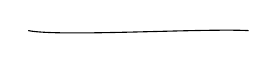
\begin{tikzpicture}\draw (0,0) .. controls (0.4,-.08) and (2.2,.03) .. (2.8,0);\end{tikzpicture}}

\margin{\uline{Leray--\unsure{Čech}}}
\diagram{\begin{tikzcd}[row sep=small] X\arrow[d,two heads]\\Y\arrow[d]\\B_F\end{tikzcd}}
$F$ un groupe, fibré principal
\[
\leftarrow\left\{\begin{gathered}\unsure{\text{d'où}}\ \text{fibration}\\\text{générale}\end{gathered}\right.
\qquad
H^*(Y)\Longleftarrow H^p(B_F,\{H^q(X)\})
\]
N.B. $\{H^q(X)\}$ est un système local \deleted{\uline{\unsure{trivial}}}\inserted{défini} par les opérations de $\pi_0(F)$ sur $H^q(X)$.
\figure{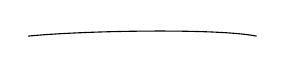
\begin{tikzpicture}\draw (0,0) .. controls (0.7,.07) and (2.4,.1) .. (2.9,0);\end{tikzpicture}}

\diagram{\begin{tikzcd}[row sep=small]Y\arrow[d,two heads]\\B_F\arrow[d]\\B_{\deleted{\unsure{G}}\inserted{X}}\end{tikzcd}}
$\deleted{\unsure{G}}\inserted{X}$ un groupe

$F$ un ss-groupe
\[
\left\{\unsure{\text{d'où}}\ \text{fibration générale}\right.
\qquad
H^*(B_F)\Longleftarrow H^{\unsure{p}}(B_{\deleted{\unsure{G}}\inserted{X}},\{H^q(Y)\})
\]
N.B. $\{H^q(Y)\}$ est un système local défini par les op. de $\pi_0(X)$ sur $H^q(X/F)$ \unsure{via celles de} $\pi_0(X)$ sur $\pi_0(X/F)$
\figure{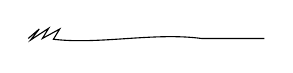
\begin{tikzpicture}\draw (0,0) -- (.14,.12) -- (.03,-.02) -- (.26,.13) -- (.18,0) -- (.4,.12) -- (.32,-.01) .. controls (.9,-.08) and (1.6,.08) .. (2.2,0) -- (3,0);\end{tikzpicture}}
\margin{\uline{Shapiro}}
Si $Y$ est discret, relation d'isomorphisme bien connue entre la coh. de $B_F$, et celle de $B_G$ à valeurs dans un coeff. \uline{induit} [à considérer surtout dans le cas où $F,G$ sont discrets]
\figure{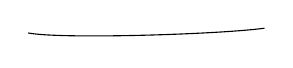
\begin{tikzpicture}\draw (0,0) .. controls (.4,-.08) and (2.4,-.02) .. (3,.06);\end{tikzpicture}}

\margin{\uline{Hochschild--Serre} $\unsure{\parallel}$ \uline{Leray--\unsure{Čech}}}
\diagram{\begin{tikzcd}[row sep=small]B_F\arrow[d,two heads]\\B_X\arrow[d]\\B_Y\end{tikzcd}}
$X$ un groupe, $F$ un ss-groupe \uline{distingué} donc $Y$ un groupe
\[
\left\{\unsure{\text{d'où}}\ \text{fibration générale}\right.
\qquad
H^*(B_G)\Longleftarrow H^p(B_Y,H^q(B_F))
\]
\scanpage{25}
% archive foliation: 24
\begin{center}- 95 -\end{center}
n° 268

variété de Picard, il nous suffira de montrer comment on peut définir de façon géométrique le passage au quotient de $A$ par le noyau de $\varphi_X$, tout en conservant certaines propriétés de rationalités, $X$ étant un diviseur non dégénéré.

Comme première application du théorème du carré, nous allons démontrer le plongement projectif d'une variété abélienne. Rappelons que si $X$ est un diviseur sur $A$ une variété $V$, complète et sans singularités de \unsure{c} codimension 1, on désigne par $\mathcal{L}(X)$ l'ensemble de tous les diviseurs positifs linéairement équivalents à $X$, et par $L(X)$ l'ensemble des fonctions $\varphi$ sur $V$ telles que $(\varphi)\geq-X$. C'est un espace vectoriel sur les constantes de dimension finie. Si $\mathcal{L}(X)$ n'est pas vide, on dit que c'est un système linéaire complet. (Cf. IAG). Si $V$ est définie sur $k$, et $X$ rationnel sur $k$, on peut trouver une base de $L(X)$ définie sur $k$.
On dit que $\mathcal{L}(X)$ \unsure{séparé|sépare} les points de $V$ si quels que soient les points $P,Q$ distincts de $V$, il existe un diviseur $Y\in\mathcal{L}(X)$ tel que $P\in\operatorname{supp}(Y)$ et $Q\notin\operatorname{supp}(Y)$. Si $\varphi_0,\ldots,\varphi_m$ est une base de $L(X)$, et $P$ est générique sur $V$ alors l'application $P\longrightarrow(\varphi_0(P),\ldots,\varphi_m(P))$ définit une application rationnelle de $V$ génériquement surjective sur une variété projective. Le système linéaire complet $\mathcal{L}$ est dit ample si l'application rationnelle est birationnelle et biholomorphe. L'existence d'un plongement projectif d'une variété normale $V$ équivaut à l'existence d'un système linéaire ample.

Ceci étant, nous avons le théorème suivant :

\uline{Théorème} 5 - Soit $A$ une variété abélienne. Alors il existe un plongement projectif de $A$, Si $X$ est un diviseur positif non dégénéré sur $A$, alors il existe un entier $m>0$ tel que $mX$ soit ample.
\scanpage{26}
% archive foliation: 25
\begin{flushright}
\uline{Familles limitées}

cf. SGA 6 $\overline{\underline{\mathrm{XIII}}}$
\end{flushright}
\scanpage{27}
% archive foliation: 26
Il y a deux \unsure{choses} à prouver

\uline{Chow raffiné} Si des $F_i$ sont quotients de \unsure{l'un} $\unsure{\simeq}L$, et \unsure{dont} les cycles associés, de \unsure{dimension} $d$, de degré borné, alors, les $F_i$ sont limités
\figure{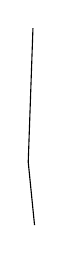
\begin{tikzpicture}\draw (0,0)--(-.06,-1.7)--(.02,-2.5);\end{tikzpicture}}

\deleted{On peut supposer $L=\underline{O}(m)^h$ et par \unsure{$L=\underline{O}^k$}}
En effet, longueur gén. de $F_i$ est à priori bornée, on \unsure{récure} sur le sup. de \deleted{\unsure{ses}}\inserted{ces} longueurs, soit $l$.
Si $l\leq0$, rien à prouver, supposons $\unsure{l\geq1}$.
\deleted{Il \unsure{existe une} \illegible{3}}\inserted{\unsure{pour} $l=1$, alors les} \unsure{énoncés} \unsure{ci-dessus}, \unsure{rien} \deleted{\unsure{à faire}} car \unsure{l'union de|l'un des} \unsure{collections} de faisceaux qui sont limités, \deleted{\unsure{sont}} \unsure{limité|limitée}.
\margin{\textcircled{e}}

Si $l=1$, $F_i\subset\deleted{\unsure{\operatorname{im}}}\underline{O}_{Z_i}$, $Z_i$ un cycle de \deleted{degré} irréductible de degré \deleted{\unsure{\text{cst.}}}\inserted{borné}. Si \deleted{les \unsure{résu}} \deleted{On} \unsure{a} prouvé que les $\underline{O}_{Z_i}$ sont limités, \unsure{il en sera} fini (les uns \unsure{images} d'hom. \unsure{variables} du faisceau $L$ dans $\underline{O}_{Z_i}$). $\unsure{\iota}$
\margin{\textcircled{d}}

Or pour ce dernier fait, on utilise Chow grossier,
\margin{\textcircled{f}}
\scanpage{28}
% archive foliation: 27
faisceaux $F_i$ quotients d'un faisceau donné $\unsure{E|L}$, et \deleted{des}\inserted{les} $P_{F_i}$ en \deleted{\unsure{nombre}}\inserted{\unsure{nb}} finis. On veut prouver que les $(F_i)$ sont limités. \deleted{\unsure{Récurrence}}

\deleted{\unsure{sur}} \unsure{a)|4°)} Résultat de Chow : les \uuline{cycles} de $P^n_{\unsure{Z|\mathbf Z}}$ de \deleted{dimension $d$} degré \deleted{\unsure{fixé}} borné sont inclus dans des fibres d'un
\diagram{\begin{tikzcd}\arrow[r,hook,"{\deleted{\unsure{\longrightarrow}}}"]&\deleted{\unsure{P^n}}\arrow[r,"{\deleted{\unsure{\longrightarrow}}}"]&\deleted{\unsure{T}}\end{tikzcd}}
morphisme \deleted{\unsure{de}}
\diagram{\begin{tikzcd}\Gamma\arrow[r,hook]&P^{\unsure{n}}_{\unsure{T}}\arrow[r]&T\end{tikzcd}}
où $T$ de type fini sur $Z$

\deleted{\unsure{On}} On procède par récurrence ascend. $*$ sur $\sup\dim\operatorname{supp}F_i=d$, le résultat est trivial si $d<0$. Si $d\geq0$, on regarde les \deleted{\unsure{F}} suites exactes
\diagram{\begin{tikzcd}0\arrow[r,no head]&F''_i\arrow[r,no head]&F_i\arrow[r,no head]&F'_i\arrow[r,no head]&0\end{tikzcd}}
\deleted{\unsure{donc}} où $\dim F''_i<d$ et $F'_i$ \deleted{\unsure{n'a que les points} \unsure{génériques de dim}} cycles associés de dim $d$.
Les $F'_i$ sont quotients de $L$, \uline{de degrés majorés}

Si on prouve qu'ils sont limités, on en conclut que les \deleted{\unsure{pol.}} $P_{F'_i}$ sont en nb fini; donc on a les
\[
P_{F''_i}=P_{F_i}-P_{F'_i}
\]
en nb fini; d'autre part les noyaux de tous les $F'_i$ sont limités, donc quotients d'un $\simeq L''$, donc les $F''_i$ sont quotients d'un $\simeq L''$ et leurs pol. de Hilb en nb fini, donc \deleted{\unsure{les uns sont tous}} grâce à l'hyp. de recurrence ils sont limités. Donc les extensions $F_i$ de $F'_i$ par $F''_i$ sont limités
\margin{\textcircled{d}}
\margin{\textcircled{e}}
\scanpage{29}
% archive foliation: 28
\uline{Définition} 1. Soient $X$ un préschéma \deleted{\unsure{de}} sur un corps $k$, $F_i$ \deleted{et $G$} $(i=1,2)$ un faisceau algébrique sur $X_i=X\otimes_kK_i$, où $K_i$ est une extension de $k$. On dit que $F_1$ et $F_2$ sont \uline{$\unsure{K|k}$-équivalents} s'il existe une extension $K'$ de $k$, des $k$-hom $u_i:K_i\longrightarrow K'$, tels que \deleted{un isomorphisme} les faisceaux algébriques \inserted{$F_i\otimes_{K_i}K'$} sur $X\otimes_kK'\simeq X_i\otimes_{K_i}K'$ soient isomorphes. \deleted{Les classes d'équivalence} Classes géométriques de faisceaux.
\figure{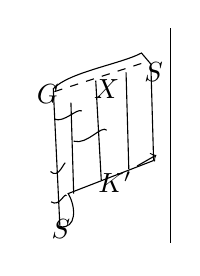
\begin{tikzpicture}[scale=.7]
\draw (0,0)..controls (.3,-.05) and (.3,.35)..(.15,.6)--(1.7,1.2);
\draw (0,0)--(-.12,2.5)..controls (.15,2.8) and (1.1,2.95)..(1.48,3.15)--(1.65,2.95)--(1.7,1.2);
\draw[dashed] (-.1,2.45)--(1.6,3);
\draw (.25,.6)--(.2,2.25);\draw (.75,.85)--(.65,2.65);\draw (1.25,1.05)--(1.2,2.8);
\draw (-.1,1.95)..controls (.08,1.88) and (.3,2.15)..(.4,2.1);
\draw (.25,1.55)..controls (.5,1.48) and (.75,1.85)..(.85,1.75);
\draw (-.17,1)..controls (-.02,.85) and (.08,1.2)..(.1,1.15);
\draw (-.16,.45)..controls (0,.35) and (.08,.63)..(.12,.56);
\draw[->] (1.4,1.1)--(1.75,1.3);
\node at (.85,2.5) {$X$};\node at (1,.8) {$K'$};
\node at (-.22,2.4) {$\unsure{G}$};\node at (1.7,2.8) {$\unsure{S}$};\node at (.02,-.05) {$\unsure{S}$};
\draw (2,3.6)--(2,-.3);
\end{tikzpicture}}

On vérifie facilement que c'est là une \uline{relation d'équivalence} entre \deleted{faisceaux}\inserted{couples $(K,F)$} d'une ext. $K$ de $k$ et d'un faisceau algébrique $F$ sur $X\otimes_kK$, en vertu du fait de transitivité de l'extension des scalaires et du fait que deux extensions de $k$ peuvent toujours être ``dominées'' par une troisième.

\uline{Proposition 2} \inserted{Si $X$ est de type fini sur $k$,} Tout faisceau cohérent sur un $X\otimes_kK$ est équivalent à un faisceau algébrique sur un $X\otimes_kK'$, où $K'$ est une ss-extension de $K$ de type fini sur $k$.

Si $F_1$ sur $X\otimes_kK_1$ et $F_2$ sur $X\otimes_kK_2$ sont des faisceaux cohérents \uline{équivalents}, \deleted{\unsure{alors}}\inserted{les $K_i$ de type fini sur $k$,} \deleted{\unsure{deux de type fini}} alors dans
\scanpage{30}
% archive foliation: 29
définition 1 on peut prendre le $K'$ une extension de \uline{type fini} de $K$.

Cela résulte de Chap V, § 1. Question : peut-on prendre pour $K'$ n'importe quelle extension \uline{\unsure{composée|commune}} ?

Cela montre que pour étudier les \deleted{\unsure{objets}} classes de faisceaux \inserted{sur $X$}, à équivalence près, on peut se borner aux faisceaux ``définis'' sur des extensions de type fini de $k$.
Cela prouve aussi \deleted{\unsure{que}} \inserted{qu'il est raisonnable de parler de classes} de classes de faisceaux à isom. près [qui est un ensemble dans le $\unsure{\mathcal U}$-univers \unsure{que} \unsure{alors|choisi} contenant $k,X$]. \inserted{$\unsure{\Phi|\mathrm{Cl}}(X/k)$}

\deleted{De plus, cet \unsure{ens} ne change pas par extension du corps de base $k$ en un $k'$. Enfin, $\unsure{\Phi|\mathrm{Cl}}(X/k)$ est un foncteur contravariant en $X\unsure{/k}$, pour $k$ fixé.}
\deleted{\uuline{Définition}}
\figure{\begin{tikzpicture}\draw (0,2)--(1.3,.1);\draw (2,2)..controls (2.5,1) and (3,.4)..(3.3,.2);\draw (4,2)..controls (4.4,1) and (4.8,.1)..(5,.2);\draw (5.8,2.3)--(6.4,.5);\draw (-.2,1.8)--(-.2,-.4);\draw (-.3,-.3)--(6.4,0);\end{tikzpicture}}
\margin{plus bas \unsure{après}}
On note que \unsure{l'ens} $\unsure{\Phi|\mathrm{Cl}}(X/k)$ est, pour \uline{$k$ fixé}, un foncteur contravariant en $X$. Cependant, si $k'$ est une extension de $k$, il n'y a pas en
\scanpage{31}
% archive foliation: 30
\uline{Corollaire 3} Soit $\widetilde{k}$ une extension algébrique close de $k$ de degré de transcendance infini, et soit $\widetilde X=X\otimes_k\widetilde k$. Alors l'ens $\unsure{\Phi|\mathrm{Cl}}(X/k)$ \deleted{\unsure{ident}} est en correspondance biunivoque avec l'ens des classes de faisceaux \inserted{coh.} $F$ sur $\widetilde X$ par l'équivalence \deleted{\unsure{suivante :} $F$ et} qui est définie \unsure{comme} suit. $F$ et $G$ sont $k$-équivalents ssi il existe un automorphisme $\sigma$ de $\widetilde k/k$ tel que ($\sigma_{\widetilde X}$ désigne l'automorphisme $\operatorname{id}_X\times\sigma$ qu'il définit sur $\widetilde X$)
\[
F\simeq\sigma_{\widetilde X}(G).
\]
En d'autres termes $\unsure{\Phi|\mathrm{Cl}}(X/k)$ est l'ens quotient de l'ens des classes à isom près de faisceaux coh. sur $\widetilde X$, par le groupe $\operatorname{Aut}(\widetilde k/k)$ y opérant de façon évidente.

Ceci dit, soit $\unsure{n|h}$ un entier, et $\unsure{\mathfrak P|\Pi}$ une \deleted{propriété}\inserted{condition} qui associe, à un \unsure{$n$-uple} de faisceaux cohérents sur un préschéma algébrique $X$ sur un corps \deleted{\unsure{alg.}} alg. clos,
\margin{\unsure{Se donner} $X$ et $\unsure{Y}$ sur $k$ \unsure{donné}, et pour $\forall\ K/k$ \unsure{donné} (\unsure{pas!} alg. clos) se donner \unsure{un} \unsure{fonction|foncteur} de $\unsure{\Psi}(X\otimes_kK)$ dans $\unsure{\Phi}(Y\otimes_kK)$, \unsure{compatibles} \deleted{\unsure{déf}} \illegible{2} \unsure{aux extensions de} $k$ \unsure{base}.}
\scanpage{32}
% archive foliation: 31
un \uline{ensemble} $T(F_1,-,F_n)$ de \deleted{des} faisceaux \inserted{cohérents} sur $X$, de façon que
\margin{à \unsure{généraliser}}

(i) Si les $F_i$ sont remplacés par des $F'_i$ isomorphes, \inserted{tout faisceau $\in$} $T(F'_1,-F'_{\unsure{i|n}})$ est isom. à \deleted{\unsure{$T$}} un faisceau $\in T(F_1,-F_n)$

(ii) Compatibilité avec l'extension de la base : $T(F_1\otimes k',-F_n\otimes k')$ est (à isomorphisme près) l'ens des faisceaux $G\otimes k'$, où $G\in T(F_1,-,F_n)$.
\figure{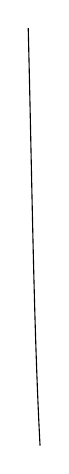
\begin{tikzpicture}\draw (0,0)..controls (.05,-2) and (.07,-3.8)..(.15,-5.3);\end{tikzpicture}}

\uline{Déf 4} Si alors $A_i$ est une partie de $\unsure{\Phi|\mathrm{Cl}}(X/k)$, $(i=1,\ldots,n)$ on désignera par $\Phi(A_1,-A_n)$ l'ens des classes \inserted{de $\unsure{\Phi|\mathrm{Cl}}(X/k)$} des él. des $\Phi(F_1,-F_n)$, où $F$ est cohérent sur $\widetilde X$ et $\operatorname{cl}_k(F_i)\in A_i$ pour tt $i$.
\figure{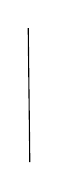
\begin{tikzpicture}\draw (0,0)--(.02,-1.7);\end{tikzpicture}}
\margin{\unsure{introduire} la \unsure{prop.} et la définition}

On voit \deleted{de \unsure{suite}}\inserted{facilement} que la définition ne change pas si on remplace $\widetilde k$ par une extension $\widetilde k'$ de $\widetilde k$ ayant les mêmes propriétés, et il est d'ailleurs facile de donner une définition directe de $\Phi(A_1,-A_n)$ sans utiliser $\widetilde k$, comme l'ens des classes
\margin{\unsure{proposition} 5}
\scanpage{33}
% archive foliation: 32
$\Phi(F_1,-F_n)$, où le $F_i$ est un faisceau coh. sur un $=X\otimes_kK$, \inserted{$K$ alg. clos,} $\operatorname{cl}_kF_i\in A_i$.

D'ailleurs, si on \uline{part} d'\deleted{\unsure{autres}} faisceaux \deleted{$K_i$} $F_i$ sur des extensions \uline{distinctes} $K_i/k$, $F_i$ de classe $\xi_i\in\unsure{\Phi|\mathrm{Cl}}(X/k)$, on obtient $\Phi(\xi_1,-\xi_n)$ en prenant de toutes les façons possibles une extension composée des $K_i$ sur $k$, et sa clôture algébrique \deleted{$K_\alpha$} $L_\alpha$, et l'on \unsure{réunit|somme} les ens de classes dans $\unsure{\Phi|\mathrm{Cl}}(X/k)$ qui correspondent à
\[
\deleted{\Phi(F_1^{(\alpha)},F_n^{(\alpha)})}\quad
\Phi(F_1\otimes_kL_\alpha,-,F_n\otimes_kL_\alpha).
\]
\margin{par le fait que les $F_i$ sont \unsure{sur|les} les \unsure{fibres} des $\Rightarrow$ \unsure{schémas|faisceaux}, $\checkmark$ \illegible{2} \unsure{qu'on a des} $\unsure{X_i-\alpha}$ \unsure{réunion}}

Si $\Phi$ est défini aussi pour des faisceaux sur un $X_K$, sans supposer $K$ alg. clos, avec validité correspondante pour (i) et (ii), alors on n'a pas besoin dans les applications précédentes de \deleted{\unsure{prendre}}\inserted{supposer les $K_i$ alg. clos}, et de passer à la clôture algébrique des extensions composées.
\scanpage{34}
% archive foliation: 33
\uline{Exemples}

a) foncteurs $\underline{\operatorname{Hom}}$, $\underline{\otimes}$, et leurs dérivés. [2 arguments, $X=Y$] \unsure{on peut regarder un argument}.

$*$ \textcircled{d} Si $F$ et $G$ sont des faisceaux, on peut \unsure{former} l'ens \inserted{$N(F,G)$} des noyaux \inserted{et $P(F,G)$} des conoyaux des hom de $F$ en $G$ [\unsure{en ce qui} $\operatorname{Im}$ ou $\operatorname{CoIm}$, c'est kif kif, mais ce dernier est contenu ds un itéré des précédents]. (2 arg, $X=Y$)

\margin{\figure{\begin{tikzpicture}[x=.45cm,y=.45cm]
\draw[->] (1,5.4) .. controls (-1,1.8) and (-.8,.9) .. (1,0);
\draw[->] (.6,-4.1) .. controls (-.5,-3.0) and (.0,-2.0) .. (1.7,-1.0);
\draw[->] (-.4,.3) .. controls (-.5,1.6) and (-.3,1.9) .. (1.4,1.9);
\end{tikzpicture}}}

b) Foncteur image inverse (1 arg, $f:X\to Y$ donné), et foncteurs dérivés

c) Foncteur image directe (1 arg. $f:X\to Y$ \unsure{propre} donné), et foncteurs dérivés

$*$ \textcircled{e} Ens. des extensions de $F$ par $G$ (2 arg, $X=Y$)

\textcircled{g} Ens des quotients associés à la filtration primaire croissante, resp. décroissante, de $F$ (1 arg, $X=Y$)

$*$ \textcircled{f} \deleted{Ens \illegible{2}} \inserted{Foncteur} $\underline O_{(\operatorname{Supp}F)_{\text{réd}}}$ ($K$ alg. clos, 1 arg, $X=Y$)

\deleted{Ens des composantes}

\textcircled{h} Ens des \deleted{\unsure{quotients}} \deleted{faisceaux} composantes primaires de $F$ associés aux composantes de son support ($K$ alg. clos, $\unsure{\chi}=0$, $X=Y$)

\deleted{\textcircled{i} \illegible{8} $F$.}
\scanpage{35}
% archive foliation: 34
\margin{\textcircled{a}\figure{\begin{tikzpicture}\draw (0,0)--(.05,-.9);\end{tikzpicture}}}
Soient $A,B\subset\Phi(X/S)$, $A$ et $B$ limités, alors $A\otimes B$ et $\operatorname{Hom}(A,B)$ sont limités, ainsi que les $\operatorname{Tor}_i(A,B)$ et $\operatorname{Ext}^i(A,B)$.

En effet, supposons
\[
\left\{\begin{aligned}
A&=\deleted{\unsure{F}}\mathcal E(F),\quad F\text{ cohérent sur }X\times_S S'\\
B&=\mathcal E(G),\quad G\quad\rule{3cm}{.2pt}\quad X\times_S S''
\end{aligned}\right.
\]
\deleted{on peut} alors considérer
\[
H=F\otimes_XG\quad\text{sur }X\times_S S''',\qquad S'''=S'\times_S S''.
\]
\margin{\diagram{\begin{tikzcd}[row sep=small,column sep=small]
&X'\arrow[dl,no head]\arrow[dd,no head]\arrow[dr,no head]&\\
X\arrow[dd,no head]&X''\arrow[l,no head]\arrow[r,no head]\arrow[ddd,no head]&X'''\arrow[dd,no head]\\
&S'\arrow[dl,no head]\arrow[dr,no head]&\\
S\arrow[dr,no head]&&S'''=S'\times_S S''\\
&S''\arrow[ur,no head]&
\end{tikzcd}}}
Alors tout type d'extension \unsure{composée} $K$ d'un $k(s')$ et $k(s'')$ sur $k(s)$ [$s'\unsure{-|\to}s$, $s''\unsure{-|\to}s$; $s'\in S'$, $s''\in S''$) provient d'un (unique) $s'''\in S'''$, $s'''\to s'$, $s'''\to s''$ et on aura
\[
(F_{s'}\otimes_{k(s')}K)\otimes_{X_{s'}\otimes_{k(s)}K}(G_{s''}\otimes_{k(s'')}K)\simeq H_{\unsure{s''|s'''}}.
\]
Comme $S'''$ est de type fini sur $S$, la conclusion pour $\otimes$ s'ensuit, on a de façon précise
\[
\deleted{\text{\unsure{Alors}}\ \mathcal E(F)\otimes}
\]
\[
\mathcal E_{X/S}(F)\otimes\mathcal E_{X/S}(G)\subset\mathcal E_{X/S}(H)
\]
Pour Hom, on \deleted{peut supposer $X'$ et $F$ $S'$-plats} \inserted{considère}
\[
\overline F=F\otimes_{S'}S'''\qquad\overline G=G\otimes_{\unsure{S'|S''}}S'''
\]
et on sait [lemme] qu'on peut trouver une \uline{partition} de $S'''$ en \inserted{\unsure{parties loc. fermées}} $T_i$ telle que, posant
\[
F_i=\overline F\otimes_{S'''}T_i=F\otimes_{S'}T_i,\qquad G_i=\overline G\otimes_{S'''}T_i=G\otimes_{\unsure{S'|S''}}T_i,
\]
\[
X_i=X'''\times_{S'''}T_i=X\times_S T_i,
\]
\scanpage{36}
% archive foliation: 35
la formation de $\underline{\operatorname{Hom}}_{X_i}(F_i,G_i)$ commute à tte extension de base $T'\unsure{-|\to}T_i$.

[pour ceci, écrire une \deleted{résolution} présentation libre de type fini
\[
L_1\longrightarrow L_0-\overline F\longrightarrow0,
\]
\deleted{puis décomposer en
\(0-Z_1-L_1-Z_0-0,\)
et \(0\longrightarrow Z_0\longrightarrow L_0-\overline F-0\)
et prendre les $Z_i$ \unsure{plats puis}}
de sorte qu'on est ramené à regarder
\[
\operatorname{Ker}\bigl(\underline{\operatorname{Hom}}(L_0,F)\longrightarrow\underline{\operatorname{Hom}}(L_1,F)\bigr),
\]
et par un lemme général on peut trouver une décomposition \inserted{de $S'''$} en des $T_i$, telle que, se restreignant à $T_i$, la formation du Ker commute au changement de base quelconque. La conclusion comme plus haut.

\margin{Rédiger sous forme de \unsure{lemme}; les $L_i$ ne \deleted{\unsure{peuvent}} \unsure{être} trouvés que \uline{localement} sur $X$. Il y a lieu de donner un lemme général \unsure{utilisable|valable} en IV, §3.}

Le cas des $\operatorname{Tor}_i$ et $\operatorname{Ext}^i$ est analogue, on est ramené au \unsure{lemme} que voici

\uline{Lemme} Soit $Y$ de type fini sur $T$ noeth, $K$ un complexe de faisceaux cohérents, à op. de degré $+1$ pour fixer les idées, $N$ un entier. Alors il y a une décomposition de $T$ en des $T_i$ loc fermés \inserted{disjoints} telle que
\scanpage{37}
% archive foliation: 36
\deleted{pour tout} posant $K^{(i)}=K\times_T T_i$, pour tt $T'$ sur $T_i$, le morphisme canonique
\[
H^q(K^{(i)}\otimes_{T_i}\unsure{T'_i|T'})\longleftarrow H^q(K^{(i)})\otimes_{T_i}T'
\]
soit un isomorphisme pour $|q|\leq N$.

Démonstration par récurrence noethérienne sur $T$, on est ramené à prouver qu'il existe un ouvert $U$ non vide de $T$ ayant la propriété des $T_i$, \inserted{$T$ étant supposé réduit.} Pour ceci, on \deleted{considère les \unsure{sous-faisceaux}} \inserted{choisit $U$ tel que les $B_i\otimes_TU$ \deleted{$\unsure{K_i}$} et $K_i$} \deleted{(cobords) $\times_TU$ \unsure{et les} soient $U$-plats pour $i$ \inserted{$|i|\leq N+1$} [$U$ étant pris avec la structure induite]} \unsure{donc} \unsure{sont} $U$-plats, pour $|i|\leq N+1$ ---

\margin{\diagram{\begin{tikzcd}[column sep=small,row sep=small]
K_{\unsure{i}}\arrow[r,"d_i"]&K_{i+1}\arrow[r,"d_{i+1}"]&K_{i+2}\\
&\unsure{H|B}_{i+1}&
\end{tikzcd}}}

\margin{\textcircled{b}\figure{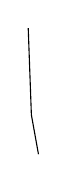
\begin{tikzpicture}\draw (0,0)--(.04,-1.1)--(.13,-1.6);\end{tikzpicture}}}
Soit $f:X-Y$ un $S$-morphisme de préschémas de type \unsure{finis}. Soit $A\subset\Phi(Y/S)$ une partie limitée, alors $f^*(A)$ et les $\operatorname{Tor}^{\underline O_Y}_{*}(A,\underline O_X)$ sont limités

Il y a intérêt à bloquer cette proposition avec la précédente, en \unsure{prenant} \deleted{\illegible{1}} $X$ et $Z$ sur $Y$, \deleted{et \illegible{1}} $A\subset\Phi(X/S)$, $B\subset\Phi(Y/S)$ et les $\operatorname{Tor}_i^{\underline O_Z}(A,B)$.
\scanpage{38}
% archive foliation: 37
Soient $X_i$ sur $Y$ ($1\leq i\leq n$), des $F_i$ sur les $X_i$, \deleted{\unsure{on a}} un changement de base $Y'-Y$, et on compare
\[
\underline{\operatorname{Tor}}_*^{\underline O_Y}(F_1,-F_n)\otimes_Y Y'\qquad\text{et}
\]
\[
\underline{\operatorname{Tor}}_*^{\underline O_{Y'}}(F'_1,-F'_n)
\]
\margin{\diagram{\begin{tikzcd}[column sep=small,row sep=large]
X_1&X_2&X'_1&X'_2\\
Y&&Y'&\\
S&&S'&
\end{tikzcd}}}

On sait qu'on a un hom canonique du premier ds le second. À quelles conditions est-ce un isomorphisme ?

\deleted{Comme le dernier \unsure{est un} \unsure{l'aboutissement}}
\deleted{\unsure{D'une}} \inserted{On a des} suites spectrales \inserted{\unsure{ab. = le dernier,|ab. le dernier,}} commençant par
\[
\operatorname{Tor}_p^{\underline O_S}\bigl(\operatorname{Tor}_q^{\underline O_Y}(F_1,-,F_n)\deleted{\otimes_Y},\underline O_{S'}\bigr),
\]
il suffit que les $\operatorname{Tor}_q^{\underline O_Y}(F_1,-,F_n)$ soient $Y$-plats.
\scanpage{39}
% archive foliation: 38
\margin{\figure{\begin{tikzpicture}\draw (0,0)--(.15,-2.8);\draw (.15,-4.6)--(.18,-5.6);\end{tikzpicture}}}
\uline{Proposition} $X_i$ ($1\leq i\leq n$) de type fini sur $Y$ de type fini sur $S$ noeth, $F_i$ coh. sur $X_i$, $N$ un entier. Alors il existe un \deleted{entier} ouvert non vide $U$ de $S$, tel que, \deleted{\unsure{désignant par}} \inserted{posant}
\[
\deleted{\unsure{U'}}\inserted{S'}=U_{\text{réd}},\quad X'_i=X\times_S\deleted{\unsure{U'}}\inserted{S'},\quad Y'=Y\times_S\deleted{\unsure{U'}}\inserted{S'},\quad F'_i=F\otimes_S S',
\]
on ait ceci : pour tout changement de base $T\longrightarrow S'$, le hom canonique
\[
\operatorname{Tor}_p^{\underline O_{S'}}(F'_1,-,F'_n)\otimes_{S'}T\longrightarrow\operatorname{Tor}_p^{\underline O_T}(F'_{1T},-,F'_{nT})
\]
(où $F'_{\alpha T}=F'_\alpha\otimes_{S'}T$) est un \uline{isom} pour $p\leq N$.

On utilise pour ceci le

\margin{\figure{\begin{tikzpicture}\draw (0,0)--(.08,-2.5);\draw (.14,-2.7)--(.2,-3.9);\draw (.25,-4.8)--(.3,-5.2);\end{tikzpicture}}}
\uline{Lemme} \inserted{Avec les notations précédentes mais sans condition de finitude,} Supposons que $Y$ soit \uline{plat} sur $S$, que les $F_\alpha$ soient plats sur $S$, et que les $\operatorname{Tor}_i^{\underline O_{\unsure{S|Y}}}(F_1,-,F_n)$ pour $i\leq N$ soient plats sur $S$. Alors pour tt changement de base $T-S$, l'hom canonique
\[
\operatorname{Tor}_i^{\underline O_S}(F_1,-,F_n)\times_S T-\operatorname{Tor}_i^{\underline O_T}(F_{1(T)},-,F_{n(T)})
\]
est un isom pour $i\leq N$.

\margin{\unsure{Peut-on faire plus ?}}
\scanpage{40}
% archive foliation: 39
\deleted{\unsure{Preuve}} Pour le prouver, on peut supposer $S$, $Y$, les $X_i$, \inserted{$T$} affines d'anneaux $A$, $B$, $B_i$, $A'$, \inserted{les} $F_i$ définis par \deleted{$M_i$} un $B_i$-module $M_i$. Soit $L^{(i)}$ une résolution libre de $M_i$ comme $B_i$-module, posons
\[
K=\mathop{\bigotimes}\limits_{1\leq i\leq n}{}_{B}L^{(i)}
\]
Alors \deleted{pour tout $i$}, les $L^{(i)}$ sont \uline{plats sur $A$}, et comme $M_i$ est plat sur $A$, il en s'ensuit que $L'^{(i)}_{\deleted{\unsure{A'}}}=L^{(i)}\otimes_A A'$ est une résolution de $M'_i=M_i\otimes_A A'$, évidemment $B'_i$-libre (où $B'_i=B_i\otimes_A A'$).

Donc la cohomologie de
\[
K'=K\otimes_A A'\deleted{\unsure{\otimes_B B'}}\inserted{{}=K\otimes_B B'}=\mathop{\bigotimes}\limits_{1\leq i\leq n}{}_{B'}L^{(i)}\otimes_B B'=\mathop{\bigotimes}\limits_{1\leq i\leq n}{}_{B'}L^{(i)'}
\]
n'est autre que $\operatorname{Tor}_{\unsure{\alpha|*}}^{B'}(M'_1,-,M'_n)$. Or comme $K$ est $A$-plat, on a une suite spectrale homologique
\[
H_{*}^{\deleted{*}}(K\otimes_A A')\Longleftarrow\operatorname{Tor}_p^A(H_q(K),A'))
\]
i.e.
\[
\operatorname{Tor}_*^{B'}(M'_1,-,M'_n)\Longleftarrow\operatorname{Tor}_p^A(\operatorname{Tor}_q^B(M_1,-,M_n),A').
\]
Il s'ensuit que si $\operatorname{Tor}_q^B(M_1,-,M_n)$ est $A$-plat pour $q\leq N$, on a l'\deleted{\unsure{établie}} isomorphisme en cause.

\margin{\diagram{$\left.\begin{tikzcd}[row sep=small,column sep=small]
M_1&M_2&\unsure{M'|M'_1}&M'_2\\
B_1&B_2&B'_1&B'_2\\
B&&B'&\\
A&&A'&
\end{tikzcd}\right\}$}}

\margin{\figure{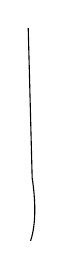
\begin{tikzpicture}\draw (0,0)--(.05,-1.9)..controls (.11,-2.3) and (.08,-2.55)..(.03,-2.7);\end{tikzpicture}}\unsure{au lieu de} la suite spectrale, on peut aussi invoquer un résultat sur la cohomologie d'un complexe.}
\scanpage{41}
% archive foliation: 40
\[
\operatorname{Tor}_p^B(M_1,-M_n)\otimes_A A'-\operatorname{Tor}_p^{B'}(M'_1,-,M'_n)
\]
est un isomorphisme pour $p\leq\unsure{n|N}$. Or c'est précisément l'hom considéré dans la proposition.

\uline{Corollaire} \inserted{Sous les conditions de la prop.} Il existe une décomposition cellulaire de $S$ en des $S_\alpha$ loc. fermés, ($1\leq i\leq n$) tels que, posant \inserted{$Y^{\alpha}=Y\times_S S_\alpha$} $X_i^{(\alpha)}=X_i\times_S S_\alpha$, $F^{(\alpha)}=F\otimes_S S_\alpha$, \deleted{\unsure{on ait pour tt}} qu'on ait ceci : pour tt changement de base $T-S_\alpha$, l'hom canonique
\[
\operatorname{Tor}_p^{\underline O_{S_\alpha}}(F_1^{(\alpha)},-,F_n^{(\alpha)})\otimes_{S_\alpha}T\longrightarrow\operatorname{Tor}_p^{\underline O_T}(F_{1(T)}^{(\alpha)},-,F_{n(T)}^{(\alpha)})
\]
est un isom pour $|p|\leq N$.

\margin{\figure{\begin{tikzpicture}\draw (0,0)--(.13,-3);\draw (.2,-4.4)--(.24,-4.75);\end{tikzpicture}}}
\uline{Proposition} $X$ de type fini sur $S$ noeth, $F$ et $G$ deux faisceaux \inserted{coh} sur $X$. \inserted{$N$ un entier.} Il existe alors une partie ouverte non vide $U$ de $S$ telle que, posant $S'=U_{\text{réd}}$, $X'=X\times_S S'$, $F'=F\times_{\unsure{S}}S'$, $G'=G\times_S S'$, l'on ait ceci : pour tt changement de base \inserted{$T\longrightarrow S$}, on a un isomorphisme
\[
\underline{\operatorname{Ext}}^p_{\underline O_{S'}}(F',G')\otimes_{S'}T\longrightarrow\underline{\operatorname{Ext}}^p_{\underline O_T}(F'_T,G'_T).
\]
pour $|p|\leq\unsure{n|N}$
\scanpage{42}
% archive foliation: 41
Résulte lui-même du

\figure{\begin{tikzpicture}[x=1cm,y=1cm]
\draw[line width=.35pt] (1.05,0) .. controls (1.12,-.65) and (1.13,-1.45) .. (1.29,-2.15);
\draw[line width=.55pt] (0,-1.35) -- (-.01,-.96) .. controls (-.04,-.80) and (.10,-.79) .. (.06,-.94) .. controls (.01,-1.02) and (-.04,-.94) .. (.01,-.87);
\end{tikzpicture}}

\uline{Lemme} \inserted{Avec les notations précédentes, mais sans conditions de finitude} Supposons que $X$ soit plat sur $S$, $F$ et $G$ plats sur $S$, \deleted{\unsure{ainsi que tt}} enfin $\operatorname{Ext}^i_{\underline O_X}(F,G)$ plat sur $S$ pour $i\leq N$, \deleted{$F$ \unsure{possède une résolution} \inserted{\unsure{libre}} \unsure{de type fini} \inserted{\unsure{libre de type fini}}} Alors pour tout $T$ sur $S$, on a des isom canoniques
\[
\operatorname{Ext}^i_{\underline O_X}(F,G)\times_S T-\operatorname{Ext}^i_{\underline O_{X_T}}(F_{(T)},G_{(T)})
\]
$i\leq N$

\margin{On suppose que pour tt $x\in X$, il existe un voisinage $U$ de $x$ tel que sur $U$, il y a une \unsure{$F$-résolution} résolution $L_*\longrightarrow F|U$ \inserted{$\leq\deleted{\unsure{N}}N+1$}, de $F|U$ de longueur $\leq N$, avec $L_i$ \unsure{libres} de type fini pour \unsure{tout} $i$ \deleted{$0\leq i\leq\unsure{N+1}$ \illegible{2}}. \deleted{$L_N$ \unsure{est de présentation finie} \unsure{pour que} $\underline{\operatorname{Hom}}(\underline L_{\unsure{N+1}},\underline{\unsure{N|G}})$, $\underline{\operatorname{Hom}}(\underline L_N,\underline{\unsure{N|G}})$ \unsure{soit aussi}, $\underline{\operatorname{Hom}}(\underline L_{N+2},\underline{\unsure{N|G}})$ soit} \uuline{$S$-plat} et
\[
\operatorname{Coker}\,\underline{\operatorname{Hom}}(\underline L_N,G)\unsure{-|\longrightarrow}\underline{\operatorname{Hom}}(\underline L_{N+1},G)
\]
$S$-plat.}

Pour définir ces isom, on suppose que $S,X,T$ sont affines, et on laisse au lecteur le soin de vérifier que les isom ainsi définis ``se recollent''.

Soient $A,B,A'$ les anneaux de $S,X,T$, $M,N$ $B$-modules qui définissent $F,G$, donc $B$ et $M$ sont $A$-plats. \inserted{Soit $B'=B\otimes_A A'$.} Soit $L_*$ un $M$-\deleted{résolution} \inserted{complexe} libre \deleted{de type fini} \inserted{de $B$-modules \unsure{libres de type fini en tous degrés}} \inserted{de longueur $\leq N+1$, et acyclique en dim $\leq N$}. \deleted{\unsure{plats et une résolution} $A$-\unsure{plate} [\unsure{résolution supposée}] \unsure{par} \unsure{$M$}} \inserted{Comme les $L_i$ et $M$ sont des $A$-modules \unsure{plats}}, $L_*\otimes_A A'$ \inserted{$=L_*\otimes_B B'$} \deleted{\unsure{est une résolution}} \inserted{\unsure{en dim} $\leq N$} \inserted{une résolution} de
\[
M\otimes_A A'=M\otimes_B B'=M',
\]
et est \unsure{libre} \deleted{\unsure{en degrés}} et de type fini en \unsure{tous degrés} \deleted{\illegible{1}}
\scanpage{43}
% archive foliation: 42
Donc on a pour $p\le N\deleted{\unsure{+1}}$
\[
\operatorname{Ext}_{B'}^p(M',N')=H^p\underline{\operatorname{Hom}}(L'_*,N')=H^p(\operatorname{Hom}_{\unsure{A|B}}(L_*,\unsure{N'|N})\otimes_A A')
\]
Soit donc $K^*=\operatorname{Hom}_{\unsure{A|B}}(L_*,N)$, dont les termes sont $A$-plats \deleted{[il suffit \unsure{en fait} que $N$ \unsure{soit} \illegible{7}]}.
On a
\[
\left.\begin{aligned}
\operatorname{Ext}_{B'}^p(M',N')&=H^p(K^*\otimes_A A')\\
\operatorname{Ext}_{B}^p(M,N)&\unsure{-|=}H^p(K^*)
\end{aligned}\right|\quad p\le N
\]
d'ailleurs les $K^i$ sont $A$-plats, les $H^p(K^*)$ aussi pour $p\le N$, et \deleted{\unsure{que}} le conoyau de $K^{\deleted{\unsure{N+1}}N}-K^{N+1}$ est $A$-plat. Il s'ensuit que l'hom canonique
\[
H^p(K^*)\otimes_A A' - H^p(K^*\otimes_A A')
\]
est un isom en \inserted{tt} degré, \deleted{\unsure{cqfd}}

en particulier pour $p\le N$ on trouve
\[
\operatorname{Ext}_{B'}^p(M',N')\xleftarrow{\sim}\operatorname{Ext}_{B}^p(M,N)\otimes_A A'
\qquad\text{cqfd.}
\]
\scanpage{44}
% archive foliation: 43
\figure{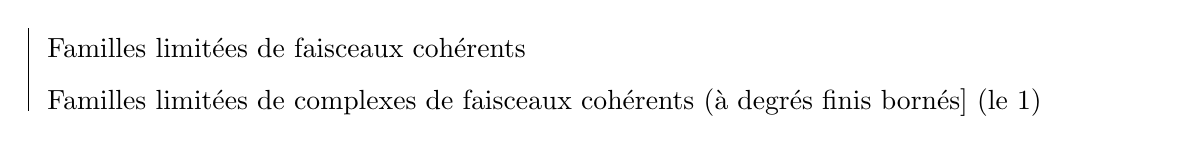
\begin{tikzpicture}
\draw (0,0.25)--(0,-0.8);
\node[anchor=west] at (0.12,0) {Familles limitées de faisceaux cohérents};
\node[anchor=north west,text width=14cm] at (0.12,-0.4) {Familles limitées de complexes de faisceaux cohérents \inserted{(\unsure{à} degrés \deleted{finis} bornés]} (\unsure{le} \illegible{1})};
\end{tikzpicture}}

\uline{Prop. 1} Réunion finie de familles limitées est limitée.

\uline{Prop 2} Possibilité dans la définition de supposer \deleted{\unsure{$S$ réduit}} des \deleted{familles} ``familles \unsure{virtuelles}'' plates sur $T$

\uline{Prop. 3} Changement de base \inserted{$S'\longrightarrow S$} transforme famille limitée en famille limitée. Réciproque si $\operatorname{Im}(S'-S)$ contient tous les points de $S$ intervenant dans $F$

\uline{Prop 4} $H^p(K)$

\uline{Prop. 5} $H^{S\,p}_{f_1,-,f_n}(K_1,-,K_n)$, si $f_i:X_i\unsure{-|\longrightarrow}X$ est propre, $K_i$ sur $X_i$.

\uline{Cor. 1} \deleted{\unsure{$L$}} Tors locaux \deleted{\unsure{$n$}}

\uline{Cor 2} Images inverses par $X'-X$

\uline{Cor 3} Images directes et $\underline{\underline R}^p f_*$

\figure{\begin{tikzpicture}\draw (0.3,0.6)--(0,0.35)--(0.8,-0.9);\end{tikzpicture}}

\uline{Prop 6} $\underline{\operatorname{Ext}}^p_{\underline O_X}(K,L)$ \hfill $[$

\uline{Cor.} $\underline{\operatorname{Hom}}(F,G)$

\uline{Prop 7} $\underline{\operatorname{Ext}}^p_{\unsure{O_X|e_X},f}(K,L)$ quand ça marche

Cor. $\underline{\operatorname{Ext}}^1_{\unsure{O_X|e_X},f}(F,G)$ en tous cas.
